\documentclass{homework}

\title{Examen}
\date{2020-07-9}
\gdate{1er Semestre 2020}
\author{Nicholas Mc-Donnell}
\course{Geometría Diferencial - MAT2305}

\setkeys{Gin}{width=.9\textwidth}

\begin{document}
\maketitle
\newpage
\pagenumbering{arabic}

\begin{sol}
    \begin{enumerate}
        \item Se denota \(\vec{x}(u,v)=\alpha(u)+v\hat{b}(u)\), se nota que como \(\alpha\) cumple que \(\kappa>0\) y es una curva entonces \(\alpha\) es \(\mathcal{C}^\infty\), al igual que \(\hat{b}\), por lo que \(\vec{x}\) es \(\mathcal{C}^\infty\). Más aún es localmente invertible en cada punto ya que \(\angled{\vec{x}_u,\vec{x}_v}=0\)\footnote{El cálculo aparece en la siguiente parte de la respuesta.}, de otra forma las columnas del Jacobiano son l.i. Con todo lo anterior, se tiene que la superficie es regular, ya que el último punto implica que \(\d{\vec{x}}\) es inyectiva y que \(\vec{x}\) localmente tiene inversa continua.
        \item Se ve lo siguiente:
              \begin{align*}
                  \vec{x}_u    & =\alpha'+v\hat{b}'   \\
                  \vec{x}_v    & =\hat{b}             \\
                  \vec{x}_{uu} & =\alpha''+v\hat{b}'' \\
                  \vec{x}_{uv} & =\hat{b}'            \\
                  \vec{x}_{vv} & =0                   \\
              \end{align*}
              Con lo anterior se calculan las formas fundamentales:
              \begin{align*}
                  E & =\angled{\vec{x}_u,\vec{x}_u}                                                                                                                   \\
                    & =\angled{\alpha'+v\hat{b}',\alpha'+v\hat{b}'}                                                                                                   \\
                    & =\angled{\alpha',\alpha'+v\hat{b}'}+\angled{v\hat{b}',\alpha'+v\hat{b}'}                                                                        \\
                    & =\angled{\alpha',\alpha'}+\angled{\alpha',v\hat{b}'}+\angled{v\hat{b}',\alpha'}+\angled{v\hat{b}',v\hat{b}'}                                    \\
                    & =\angled{\alpha',\alpha'}+2\angled{\alpha',v\hat{b}'}+\angled{v\hat{b}',v\hat{b}'}\qquad/\hat{b}'\parallel \hat{n}\text{ y }\hat{t}\perp\hat{n} \\
                    & =\norm{\alpha'}^2+v^2\norm{\hat{b}'}^2                                                                                                          \\
                    & =\norm{\hat{t}}^2+v^2\norm{-\tau\hat{n}}^2                                                                                                      \\
                    & =1+v^2\tau^2                                                                                                                                    \\
              \end{align*}
              \begin{align*}
                  F & =\angled{\vec{x}_u,\vec{x}_v}                                                                                                         \\
                    & =\angled{\alpha'+v\hat{b}',\hat{b}}                                                                                                   \\
                    & =\angled{\alpha',\hat{b}}+\angled{v\hat{b}',\hat{b}}\qquad/\hat{b}'\parallel \hat{n},\hat{t}\perp\hat{n}\text{ y }\hat{b}\perp\hat{n} \\
                    & =0                                                                                                                                    \\
                  G & =\angled{\vec{x}_v,\vec{x}_v}                                                                                                         \\
                    & =\angled{\hat{b},\hat{b}}                                                                                                             \\
                    & =\norm{\hat{b}}^2                                                                                                                     \\
                    & =1                                                                                                                                    \\
              \end{align*}
              Ahora se calcula \(\vec{x}_u\wedge\vec{x}_v\):
              \begin{align*}
                  \vec{x}_u\wedge\vec{x}_v & =(\alpha'+v\hat{b}')\wedge\hat{b}                  \\
                                           & =\alpha'\wedge\hat{b}+v\hat{b}'\wedge\hat{b}       \\
                                           & =\hat{t}\wedge\hat{b}+v(-\tau\hat{n})\wedge\hat{b} \\
                                           & =-\hat{n}-v\tau\hat{t}                             \\
              \end{align*}
              Por lo que \(\norm{\vec{x}_u\wedge\vec{x}_v}=\sqrt{1+v^2\tau^2}\), lo cual se denotará \(\lambda\) para facilitar los cálculos.
              \begin{align*}
                  N & =\frac{\vec{x}_u\wedge\vec{x}_v}{\norm{\vec{x}_u\wedge\vec{x}_v}} \\
                    & =-\frac1\lambda\paren{\hat{n}+v\tau\hat{t}}
              \end{align*}
              Ahora se calculan los coeficientes de la segunda forma fundamental:
              \begin{align*}
                  e & =\angled{N,\vec{x}_{uu}}                                                                                                                  \\
                    & =\angled{-\frac1\lambda\paren{\hat{n}+v\tau\hat{t}},\alpha''+v\hat{b}''}                                                                  \\
                    & =\angled{-\frac1\lambda\paren{\hat{n}+v\tau\hat{t}},\hat{t}'+v\paren{-\tau\hat{n}}'}                                                      \\
                    & =\angled{-\frac1\lambda\paren{\hat{n}+v\tau\hat{t}},k\hat{n}-v\tau\paren{-k\hat{t}-\tau\hat{b}}}                                          \\
                    & =\angled{-\frac1\lambda\paren{\hat{n}+v\tau\hat{t}},k\hat{n}+kv\tau\hat{t}+v\tau^2\hat{b}}                                                \\
                    & =-\frac1\lambda\paren{\angled{\hat{n},k\hat{n}+kv\tau\hat{t}+v\tau^2\hat{b}}+\angled{v\tau\hat{t},k\hat{n}+kv\tau\hat{t}+v\tau^2\hat{b}}} \\
                    & =-\frac1\lambda\paren{k+kv^2\tau^2}                                                                                                       \\
                    & =-\frac{k}\lambda\paren{1+v^2\tau^2}                                                                                                      \\
                    & =-\frac{k}\lambda\cdot\lambda^2                                                                                                           \\
                    & =-k\lambda                                                                                                                                \\
                  f & =\angled{N,\vec{x}_{uv}}                                                                                                                  \\
                    & =\angled{-\frac1\lambda\paren{\hat{n}+v\tau\hat{t}},\hat{b}'}                                                                             \\
                    & =\angled{-\frac1\lambda\paren{\hat{n}+v\tau\hat{t}},-\tau\hat{n}}                                                                         \\
                    & =\frac\tau\lambda                                                                                                                         \\
                  g & =\angled{N,\vec{x}_{vv}}                                                                                                                  \\
                    & =\angled{N,0}                                                                                                                             \\
                    & =0                                                                                                                                        \\
              \end{align*}
              Con lo que se tienen todos los coeficientes de la primera y de la segunda forma fundamental.
        \item Usando los coeficientes de las formas fundamentales se tiene lo siguiente:
              \begin{align*}
                  K & =\frac{eg-f^2}{EG-F^2}                         \\
                    & =\frac{-f^2}{EG}                               \\
                    & =-\frac{\paren{\frac\tau\lambda}^2}{\lambda^2} \\
                    & =-\frac{\tau^2}{\lambda^4}
              \end{align*}
              Ahora por el teorema de Minding se tiene que dos superficies son localmente isométricas ssi su curvatura gaussiana es igual. Ahora se nota que \(K=0\) ssi \(\tau=0\)\footnote{\(\lambda^4=\paren{1+v^2\tau^2}^2\geq1\)}, y eso quiere decir que \(S\) es localmente isométrica al plano ssi \(\alpha\) es una curva planar.
    \end{enumerate}
\end{sol}

\begin{sol}
    \begin{enumerate}
        \item Para calcular \(\tau_g\) primero se escribirá \(\hat{t}\) y \(\hat{h}\) en la base ortonormal \(\{e_1,e_2\}\)\footnote{Vectores propios de \(\d{N}\)}, sea \(\varphi\) el ángulo entre \(\hat{t}\) y \(e_1\), entonces se tiene que \(\hat{t}=e_1\cos\varphi+e_2\sin\varphi\) y como \(\hat{t}\perp\hat{h}\) se tiene que \(\hat{h}=e_1\sin\varphi-e_2\cos\varphi\). Además, se tiene que \(\frac{\d{N}}{\d{s}}=\d{N}(\hat{t})\) por lo que se tiene lo siguiente:
              \begin{align*}
                  \tau_g & =\angled{\frac{\d{N}}{\d{s}},\hat{h}}                                                                              \\
                         & =\angled{\d{N}(\hat{t}),\hat{h}}                                                                                   \\
                         & =\angled{\d{N}(e_1\cos\varphi+e_2\sin\varphi),e_1\sin\varphi-e_2\cos\varphi}                                       \\
                         & =\angled{\d{N}(e_1\cos\varphi)+\d{N}(e_2\sin\varphi),e_1\sin\varphi-e_2\cos\varphi}                                \\
                         & =\angled{e_1k_1\cos\varphi+e_2k_2\sin\varphi,e_1\sin\varphi-e_2\cos\varphi}                                        \\
                         & =\angled{e_1k_1\cos\varphi,e_1\sin\varphi-e_2\cos\varphi}+\angled{e_2k_2\sin\varphi,e_1\sin\varphi-e_2\cos\varphi} \\
                         & =k_1\cos\varphi\sin\varphi-k_2\sin\varphi\cos\varphi                                                               \\
                         & =(k_1-k_2)\sin\varphi\cos\varphi
              \end{align*}
              Llegando a lo pedido.
        \item Se nota lo siguiente:
              \begin{align*}
                  \tau_g=0 & \iff \angled{\d{N}(\hat{t}),\hat{h}}=0                    \\
                           & \iff \d{N}(\hat{t})\perp\hat{h}                           \\
                           & \iff \d{N}(\hat{t})\parallel\hat{t}                       \\
                           & \iff \d{N}(\hat{t})=\lambda(s)\hat{t}                     \\
                           & \iff \d{N}(\alpha')=\lambda(s)\alpha'                     \\
                           & \iff \text{\(\alpha\) es linea de curvatura\footnotemark} \\
              \end{align*}\footnotetext{Esto último es por Olinde-Rodrigues}
        \item Para esto se recuerda que \(k_n=k\cos\theta\) donde \(\cos\theta=\angled{\hat{n},N}\), como \(k\neq0\) se tiene que \(\hat{n}\perp N\), por lo que \(\hat{n}\in T_p(S)\), más como \(\hat{t}\perp\hat{n}\) se puede tomar \(\hat{h}\) tal que \(\hat{h}=\hat{n}\). Ahora, se tiene que \(\angled{N,\hat{n}}=0\), por lo que \(\tau_g=-\angled{N,\hat{n}'}\), desarrollándolo un poco más:
              \begin{align*}
                  \tau_g & =-\angled{N,\hat{n}'}                           \\
                         & =-\angled{N,-k\hat{t}-\tau\hat{b}}\footnotemark \\
                         & =-\angled{\hat{b},-k\hat{t}-\tau\hat{b}}        \\
                         & =-(-\tau)                                       \\
                         & =\tau                                           \\
              \end{align*}\footnotetext{\(\hat{b}=\hat{t}\wedge\hat{n}=N\)}
              Usando lo demostrado en (a) se tiene que:
              \begin{align*}
                  \tau^2 & =\tau_g^2                                              \\
                         & =\paren{(k_1-k_2)\sin\varphi\cos\varphi}^2             \\
                         & =(k_1-k_2)^2\sin^2\varphi\cos^2\varphi                 \\
                         & =\paren{(k_1+k_2)^2-4k_1k_2}\sin^2\varphi\cos^2\varphi \\
                         & =\paren{(-2H)^2-4K}\sin^2\varphi\cos^2\varphi          \\
                         & =\paren{4H^2-4K}\sin^2\varphi\cos^2\varphi             \\
                         & =4\paren{H^2-K}\sin^2\varphi\cos^2\varphi              \\
              \end{align*}
              Luego con unos cálculos formales se tiene que \(H=0\) y que \(\varphi=\frac\pi4\), por lo que \(\tau^2=-K\).
    \end{enumerate}
\end{sol}

\begin{sol}
    \begin{enumerate}
        \item Para calcular la curvatura geodésica se usará la siguiente identidad \(k^2=k_g^2+k_n^2\), se sabe que para una circunferencia de radio \(r\) se tiene que \(k=\frac1r\), más aún se sabe que en una esfera unitaria \(k_1=k_2=1\) por lo que \(k_n=1\), con esto se tiene que \(k_g=\frac{\sqrt{1-r^2}}r\).
        \item Sean \(A_i\) las regiones que no contienen el polo norte de la esfera delimitadas por los círculos de radio \(r_i\) y con centro en el plano \(XY\) tal que son tangentes a pares. Sean \(B_j\) con \(j=1,2\) las regiones triangulares restantes. Se nota que \(\iint_{S^2}1\d{\sigma}=4\pi\), que \(S^2\) es la unión disjunta de los \(B_j\) y los \(A_i\), y por último que \(\iint_{B_1}1\d{\sigma}=\iint_{B_2}1\d{\sigma}\). Dado esto se ve que el área que corresponde al triángulo en el polo norte es
              \begin{equation*}
                  \dfrac{\ds4\pi-\sum_{i=1}^3\iint_{A_i}1\d{\sigma}}2
              \end{equation*}
              Ahora, se recuerda que tras una rotación se puede parametrizar \(A_i\) con \(\vec{x}(\theta,\varphi)=\paren{\sin\theta\cos\varphi,\sin\theta\sin\varphi,\cos\theta}\) donde \(\theta\in[0,\theta_i]\)\footnote{\(\theta_i=\arccos(r_i)\)} y \(\varphi\in[0,2\pi]\). Se ve que \(E=1,F=0,G=\sin^2\theta\). Dado lo anterior se puede calcular el área de \(A_i\) con la siguiente integral:
              \begin{equation*}
                  \iint_{[0,\theta_i]\times[0,2\pi]}\sqrt{EG-F^2}\d{\sigma}
              \end{equation*}
              Reescribiendo la integral:
              \begin{align*}
                  \iint_{[0,\theta_i]\times[0,2\pi]}\sqrt{EG-F^2}\d{\sigma} & =\int_0^{\theta_i}\int_0^{2\pi}\sin\theta\footnotemark\d{\varphi}\d{\theta} \\
                                                                            & =2\pi\int_0^{\theta_i}\sin\theta\d{\theta}                                  \\
                                                                            & =2\pi\int_0^{\theta_i}\sin\theta\d{\theta}                                  \\
                                                                            & =2\pi\paren{1-\cos(\theta_i)}                                               \\
                                                                            & =2\pi\paren{1-r_i}                                                          \\
              \end{align*}\footnotetext{Se tiene que \(0\leq\theta_i\leq\frac\pi2\), por lo que \(\abs{\sin\theta}=\sin\theta\)}
              Juntando todo se tiene que el área del triángulo es:
              \begin{align*}
                  \dfrac{\ds4\pi-\sum_{i=1}^3\iint_{A_i}1\d{\sigma}}2 & =2\pi-\sum_{i=1}^3\pi(1-r_i) \\
                                                                      & =\pi\paren{r_1+r_2+r_3-1}
              \end{align*}
    \end{enumerate}
\end{sol}

\begin{sol}
    \begin{enumerate}
        \item Se nota que el toro dado es la superficie de revolución generada por la curva cerrada \(\alpha(t)=(2+\cos(t),0,\sin(t))\) respecto al eje \(Z\), por lo que los meridianos son lineas de curvatura. Además, se nota que la curva \(\gamma\) corresponde a un paralelo\footnote{Corresponde a fijar el punto \((3,0,0)\) y rotarlo respecto al eje \(Z\).}, por lo que también es una linea de curvatura.
    \end{enumerate}
\end{sol}

\begin{sol}
    \begin{enumerate}
        \item Para calcular los símbolos de Christoffel se ve lo siguiente:
              \begin{align*}
                   & \begin{cases}
                      \Gamma^1_{1 1}\cdot\frac1{y^2}+\Gamma^2_{1 1}\cdot 0=0 \\
                      \Gamma^1_{1 1}\cdot 0+\Gamma^2_{1 1}\cdot \frac1{y^2}=\frac1{y^3}
                  \end{cases} \\
                   & \begin{cases}
                      \Gamma^1_{1 2}\cdot \frac1{y^2}+\Gamma^2_{1 2}\cdot 0=\frac1{y^3} \\
                      \Gamma^1_{1 2}\cdot 0+\Gamma^2_{1 2}\cdot \frac1{y^2}=0
                  \end{cases} \\
                   & \begin{cases}
                      \Gamma^1_{2 2}\cdot \frac1{y^2}+\Gamma^2_{2 2}\cdot 0=0 \\
                      \Gamma^1_{2 2}\cdot 0+\Gamma^2_{2 2}\cdot \frac1{y^2}=\frac1{y^3}
                  \end{cases} \\
              \end{align*}
            Por lo que \(\Gamma^1_{1 1}=\Gamma^2_{1 2}=\Gamma^1_{2 2}=0\) y \(\Gamma^2_{1 1}=\Gamma^1_{1 2}=\Gamma^2_{2 2}=\frac1y\). Ahora como \(F=0\) se puede usar la siguiente identidad demostrada en tarea:
            \begin{align*}
                K&=-\frac1{2\sqrt{EG}}\paren{\paren{\frac{E_y}{\sqrt{EG}}}_y+\paren{\frac{G_x}{\sqrt{EG}}}_x}
            \end{align*}
            Se desarrolla lo anterior:
            \begin{align*}
                K&=-\frac1{2\sqrt{EG}}\paren{\paren{\frac{E_y}{\sqrt{EG}}}_y+\paren{\frac{G_x}{\sqrt{EG}}}_x}\\
                &=-\frac12y^2\paren{\paren{\dfrac{\frac{-2}{y^3}}{\frac1{y^2}}}_y+\paren{\dfrac{0}{\frac1{y^2}}_x}}\\
                &=-\frac12y^2\paren{\dfrac{-2}{y}}_y\\
                &=-\frac12y^2\dfrac{2}{y^2}\\
                &=-1\\
            \end{align*}
    \end{enumerate}
\end{sol}


% \section*{Apéndice}
% \begin{center}
%     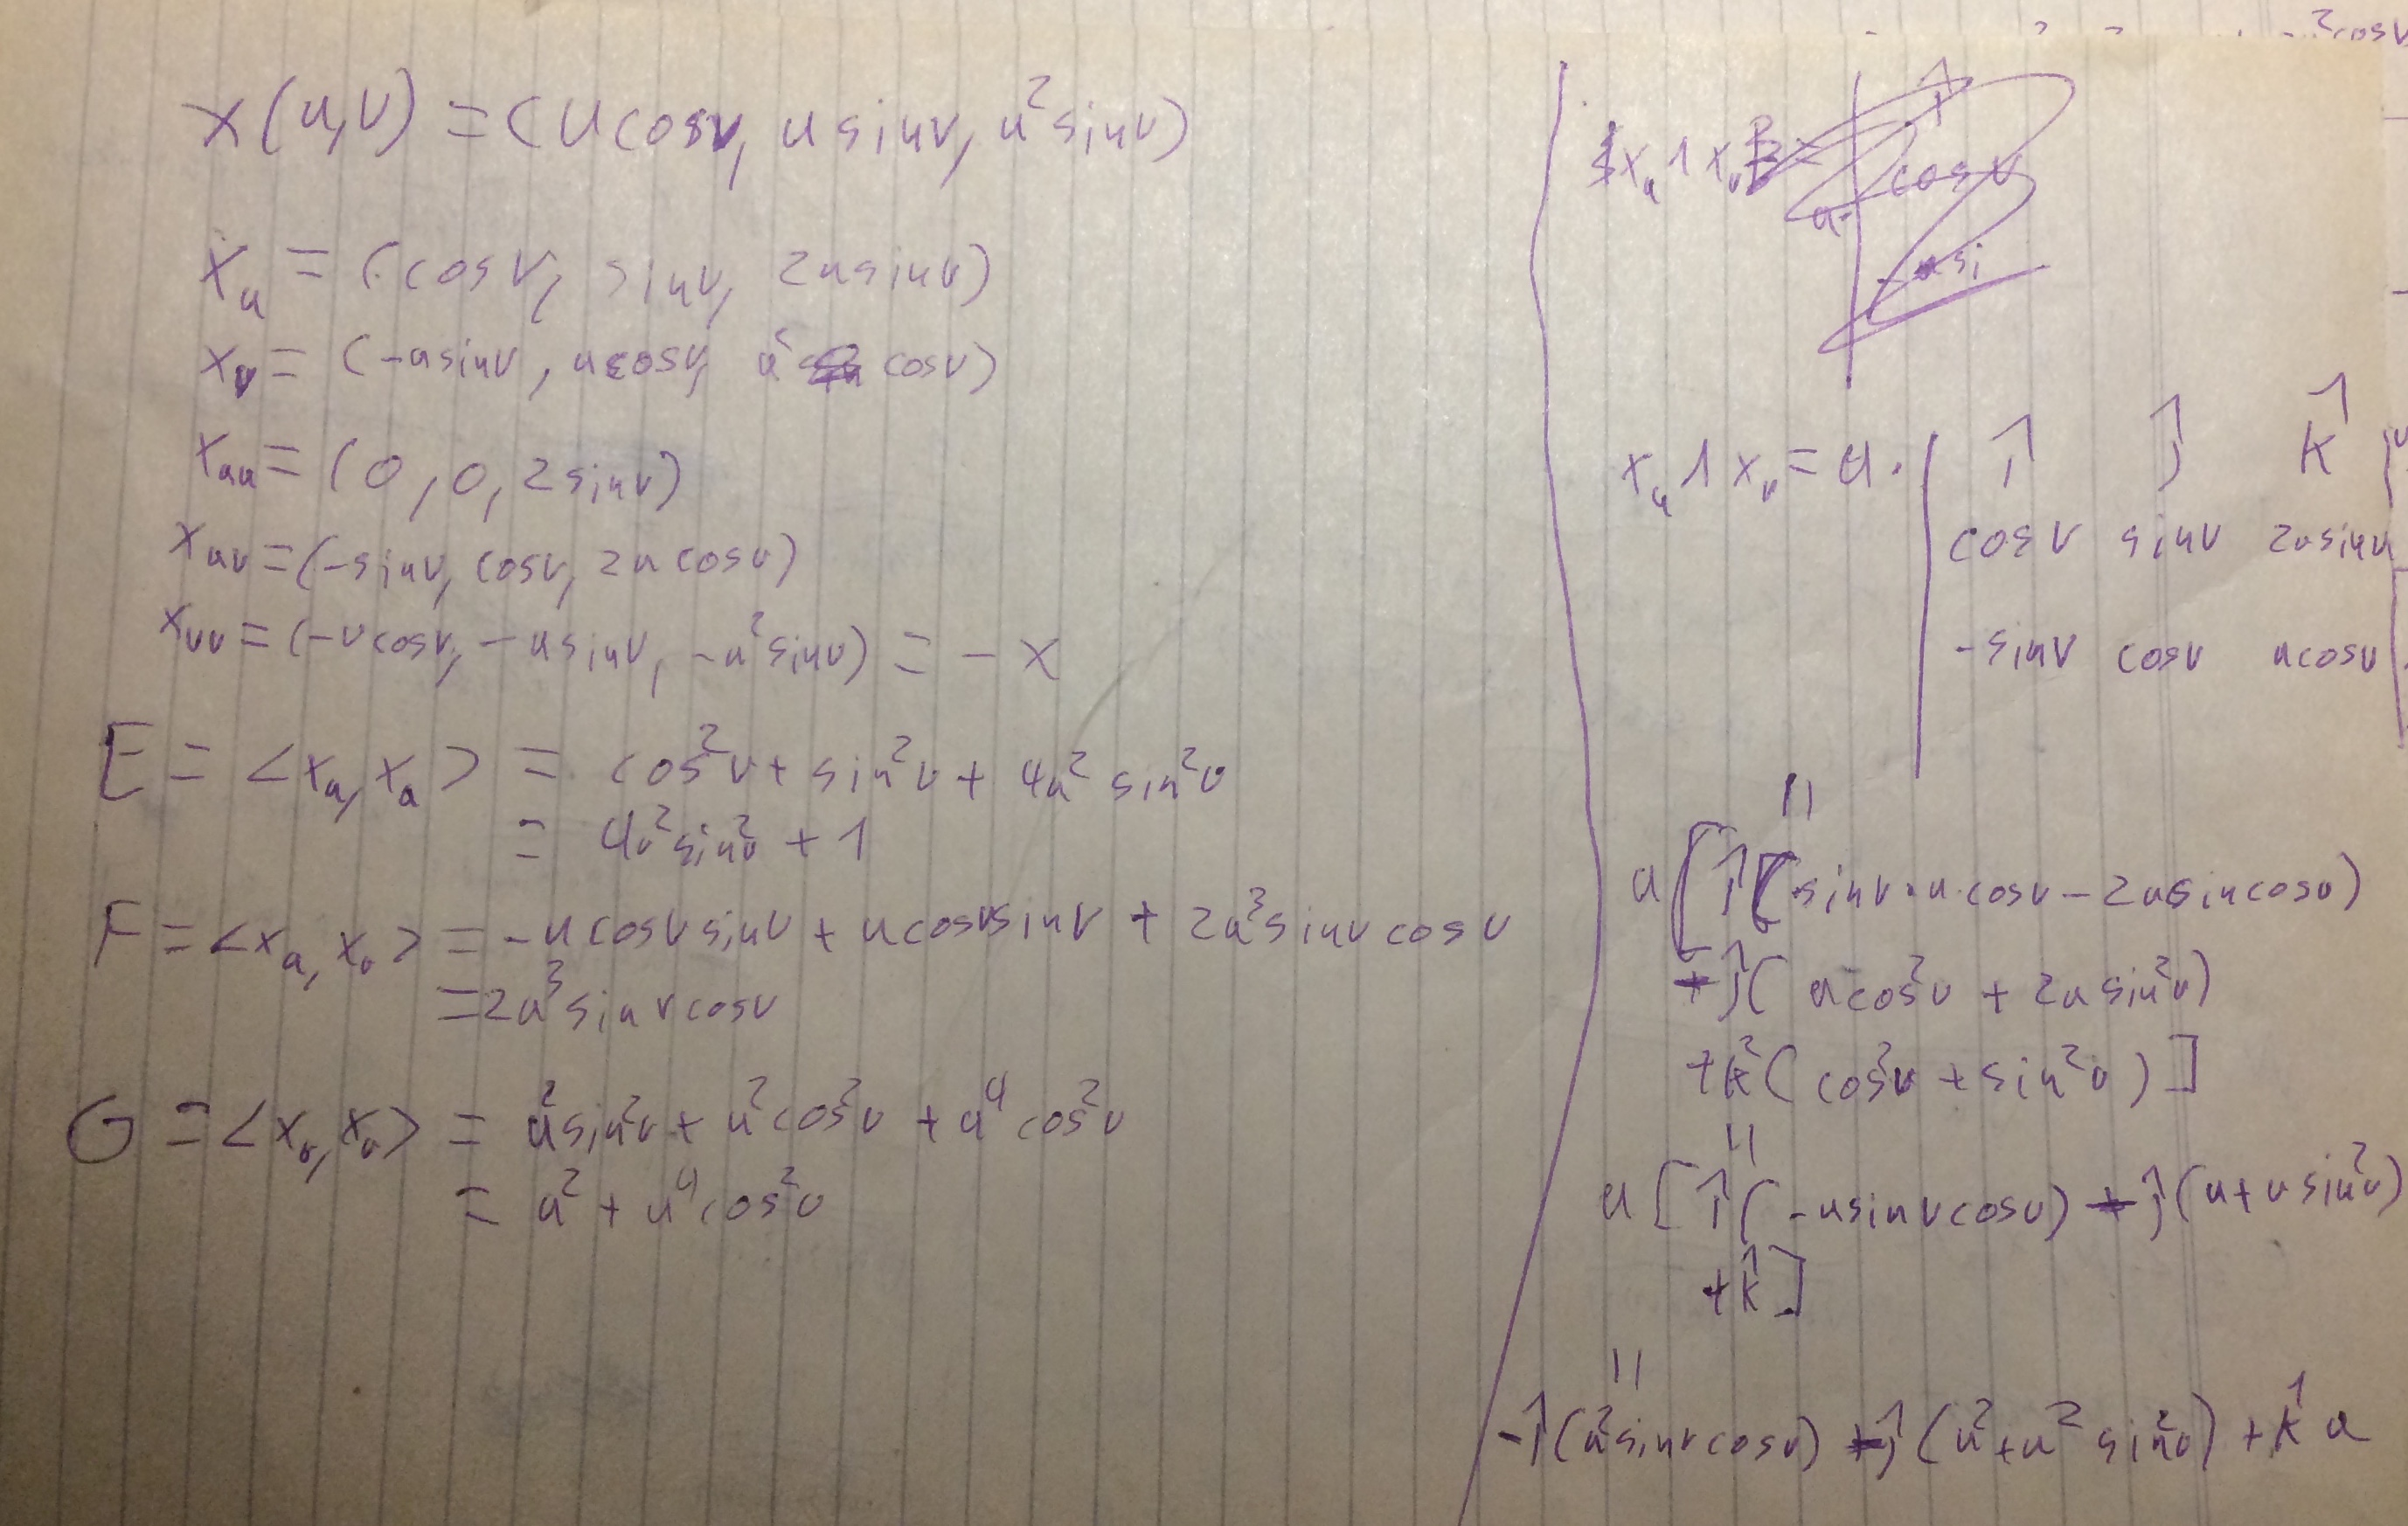
\includegraphics{img/IMG_5982.JPG}
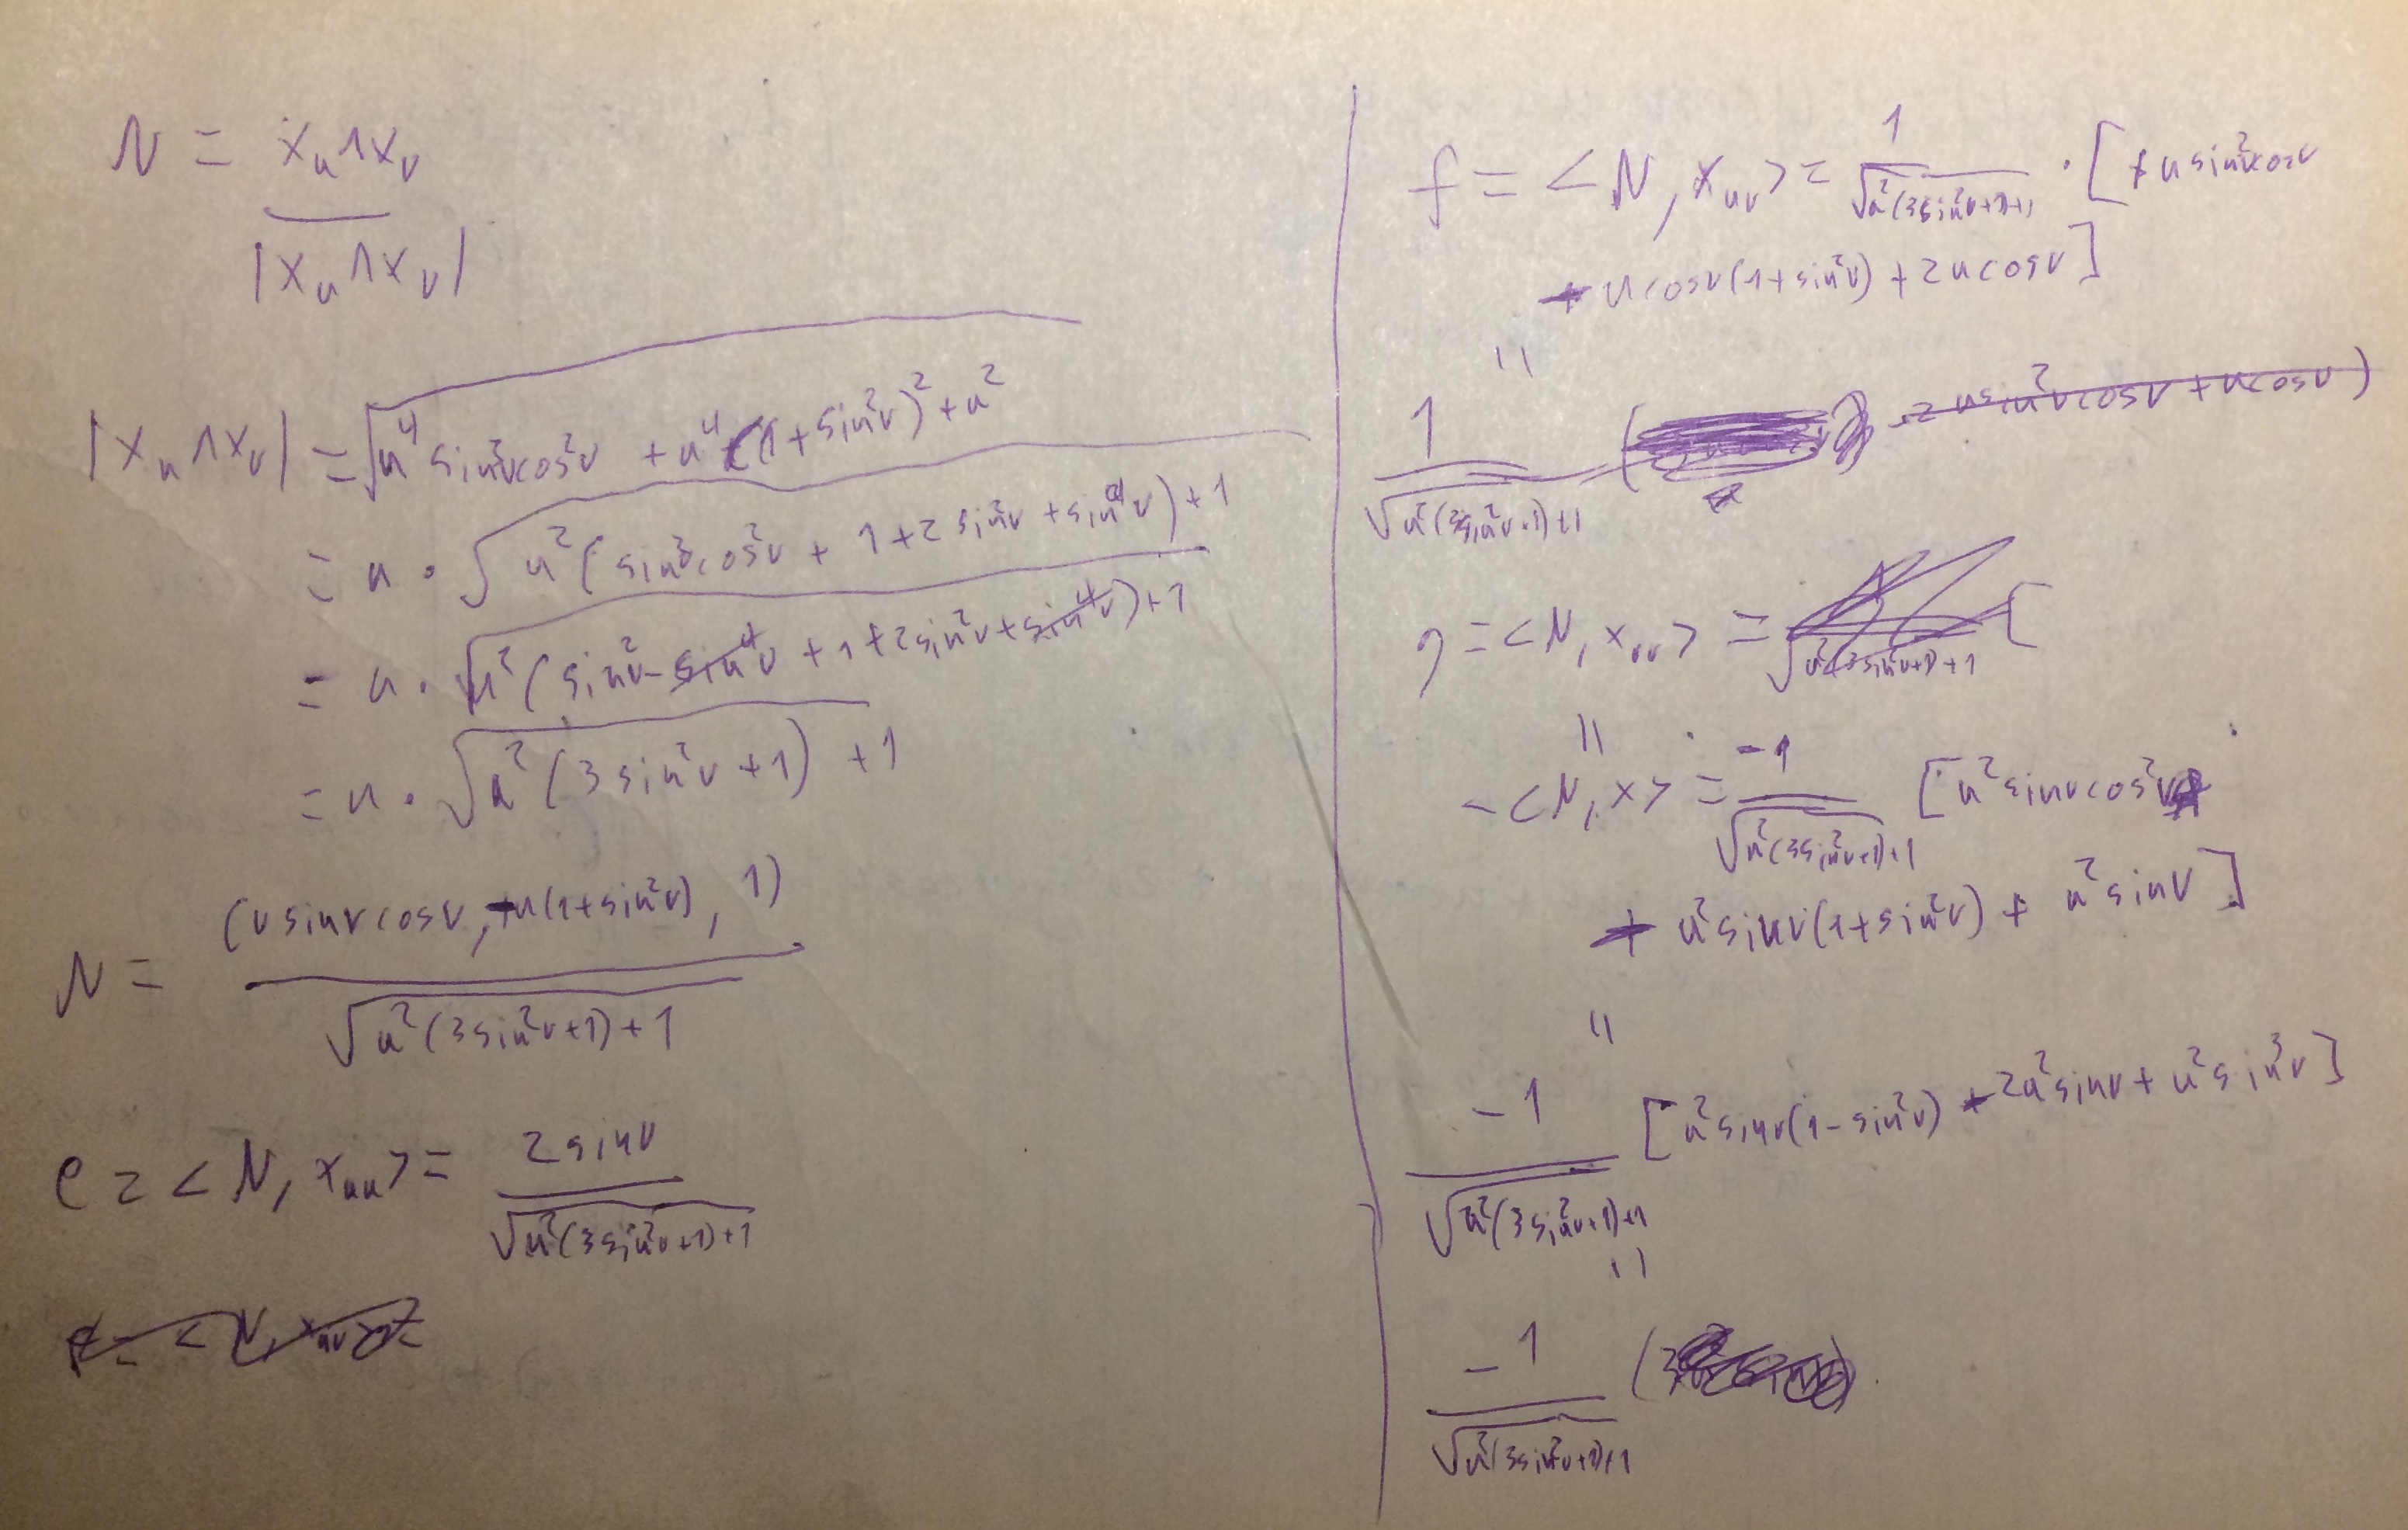
\includegraphics{img/IMG_5983.JPG}
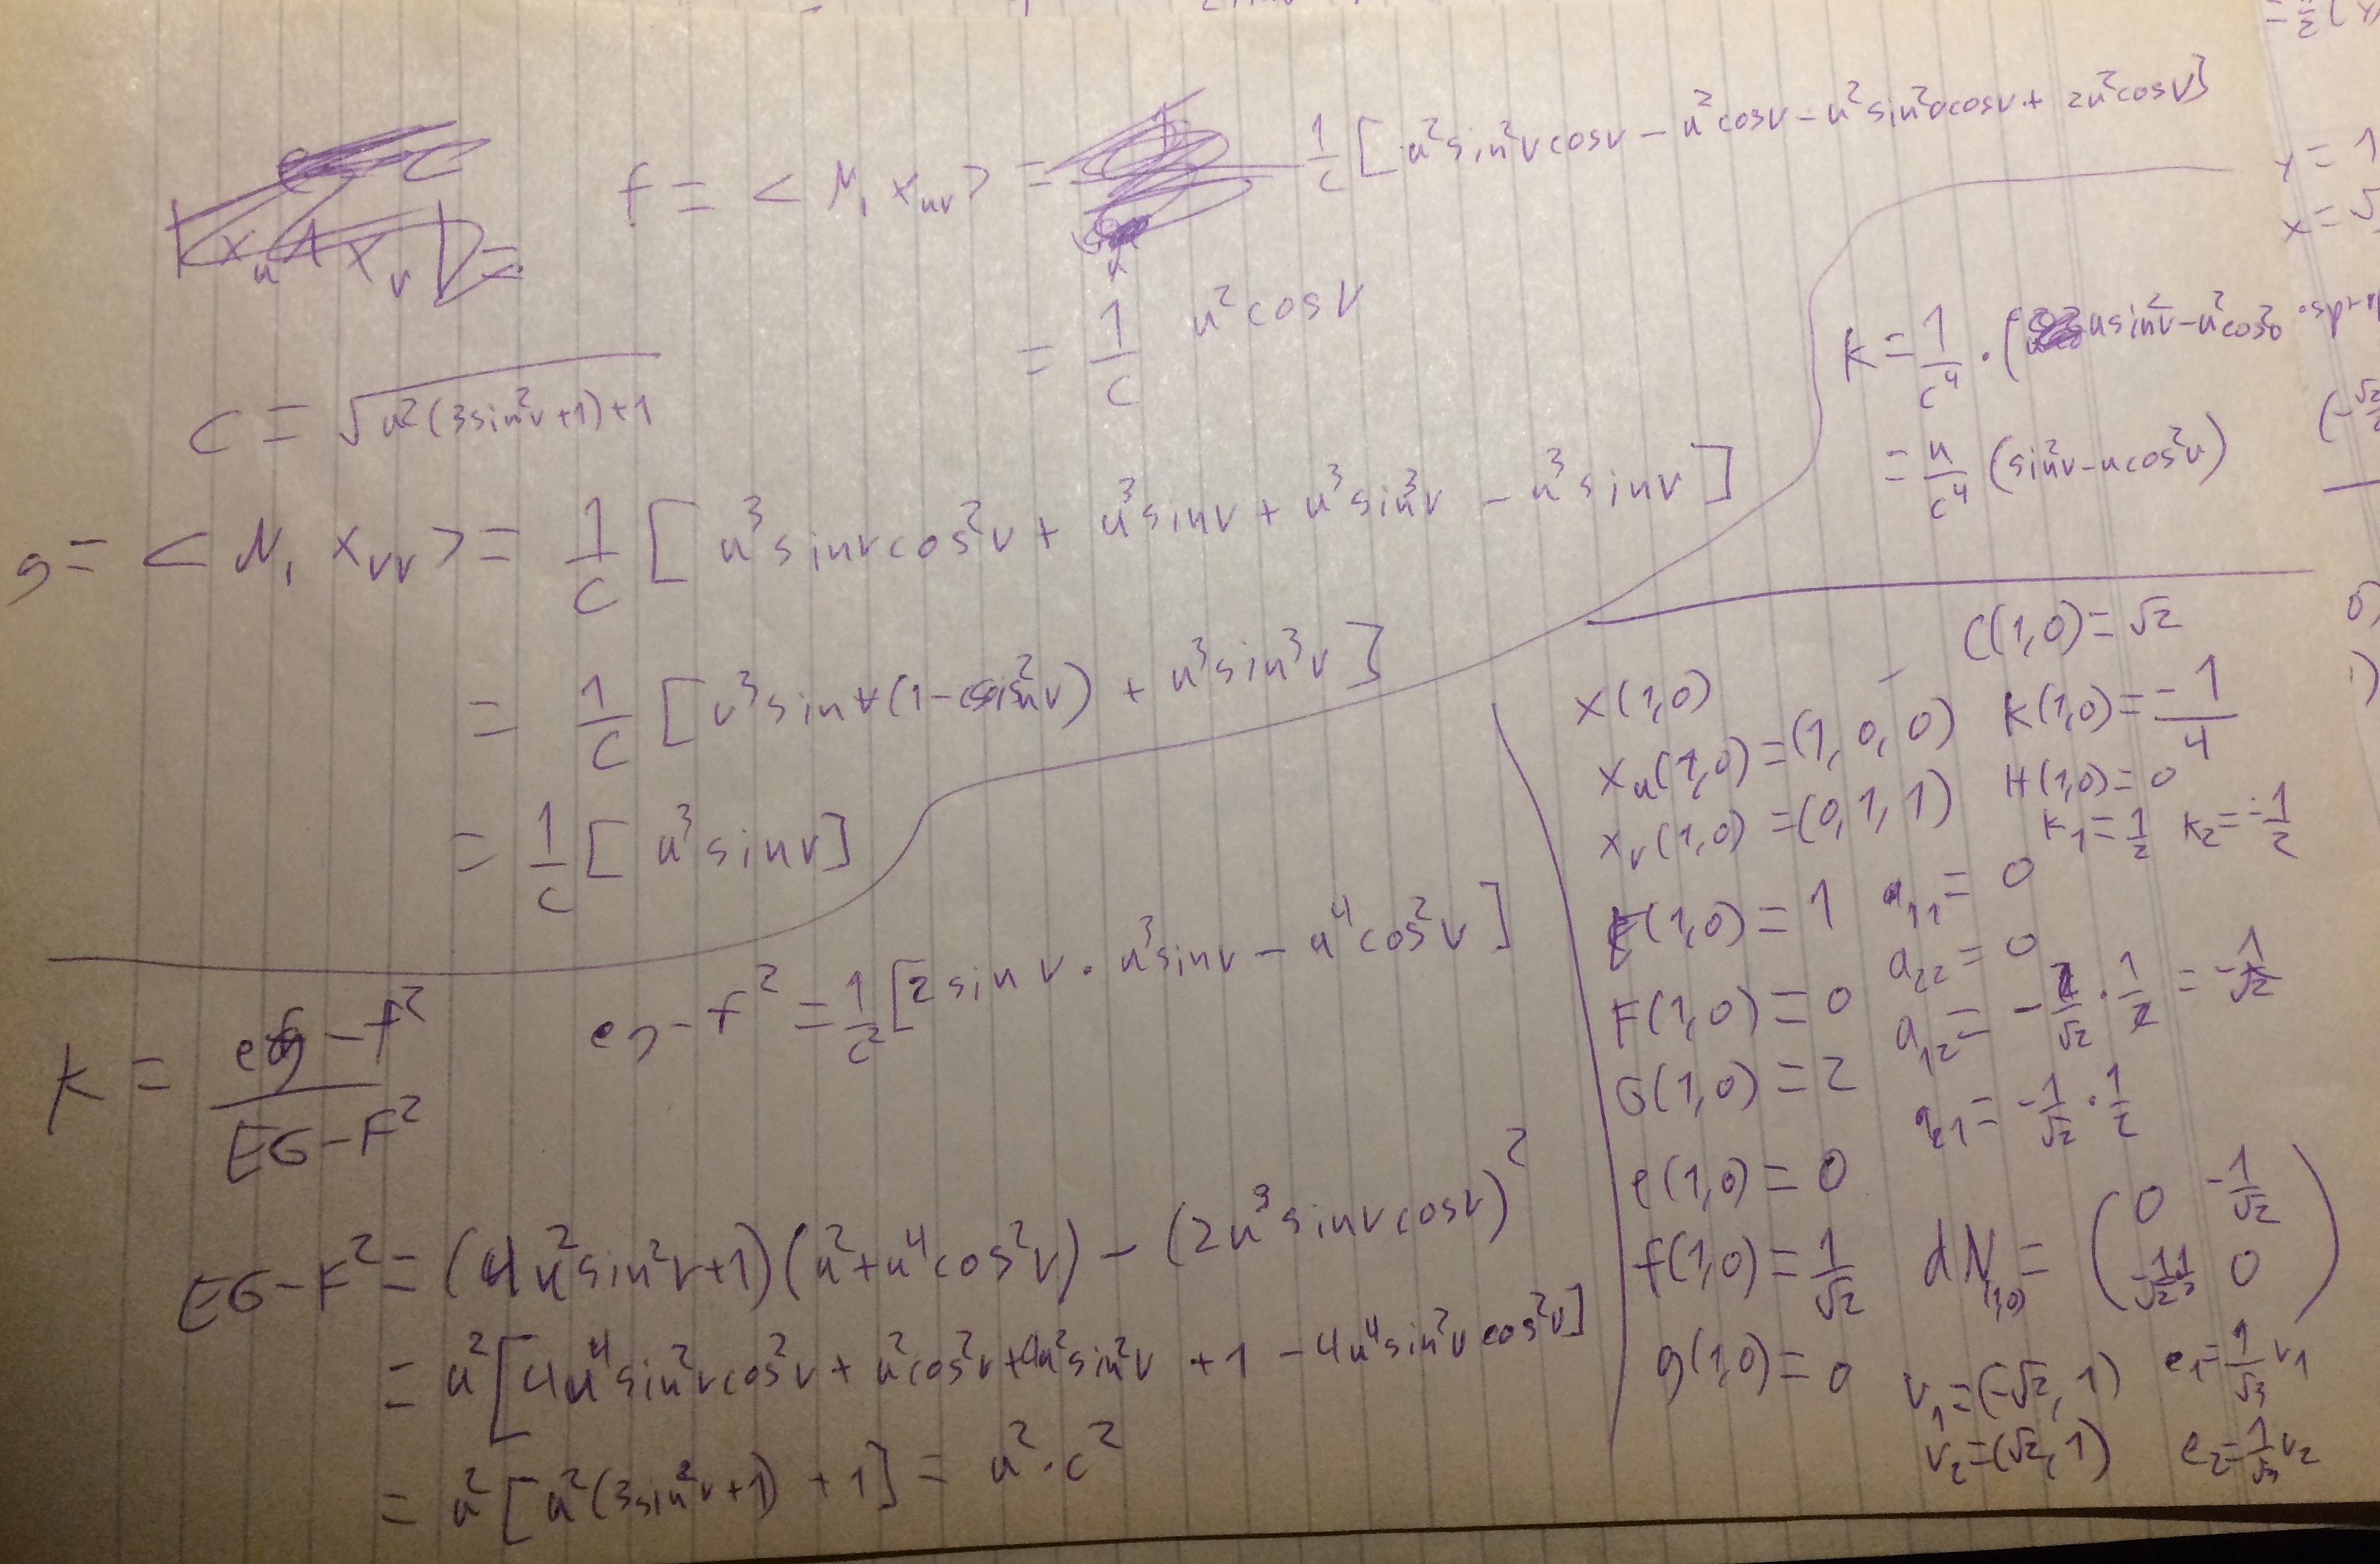
\includegraphics{img/IMG_5984.JPG}
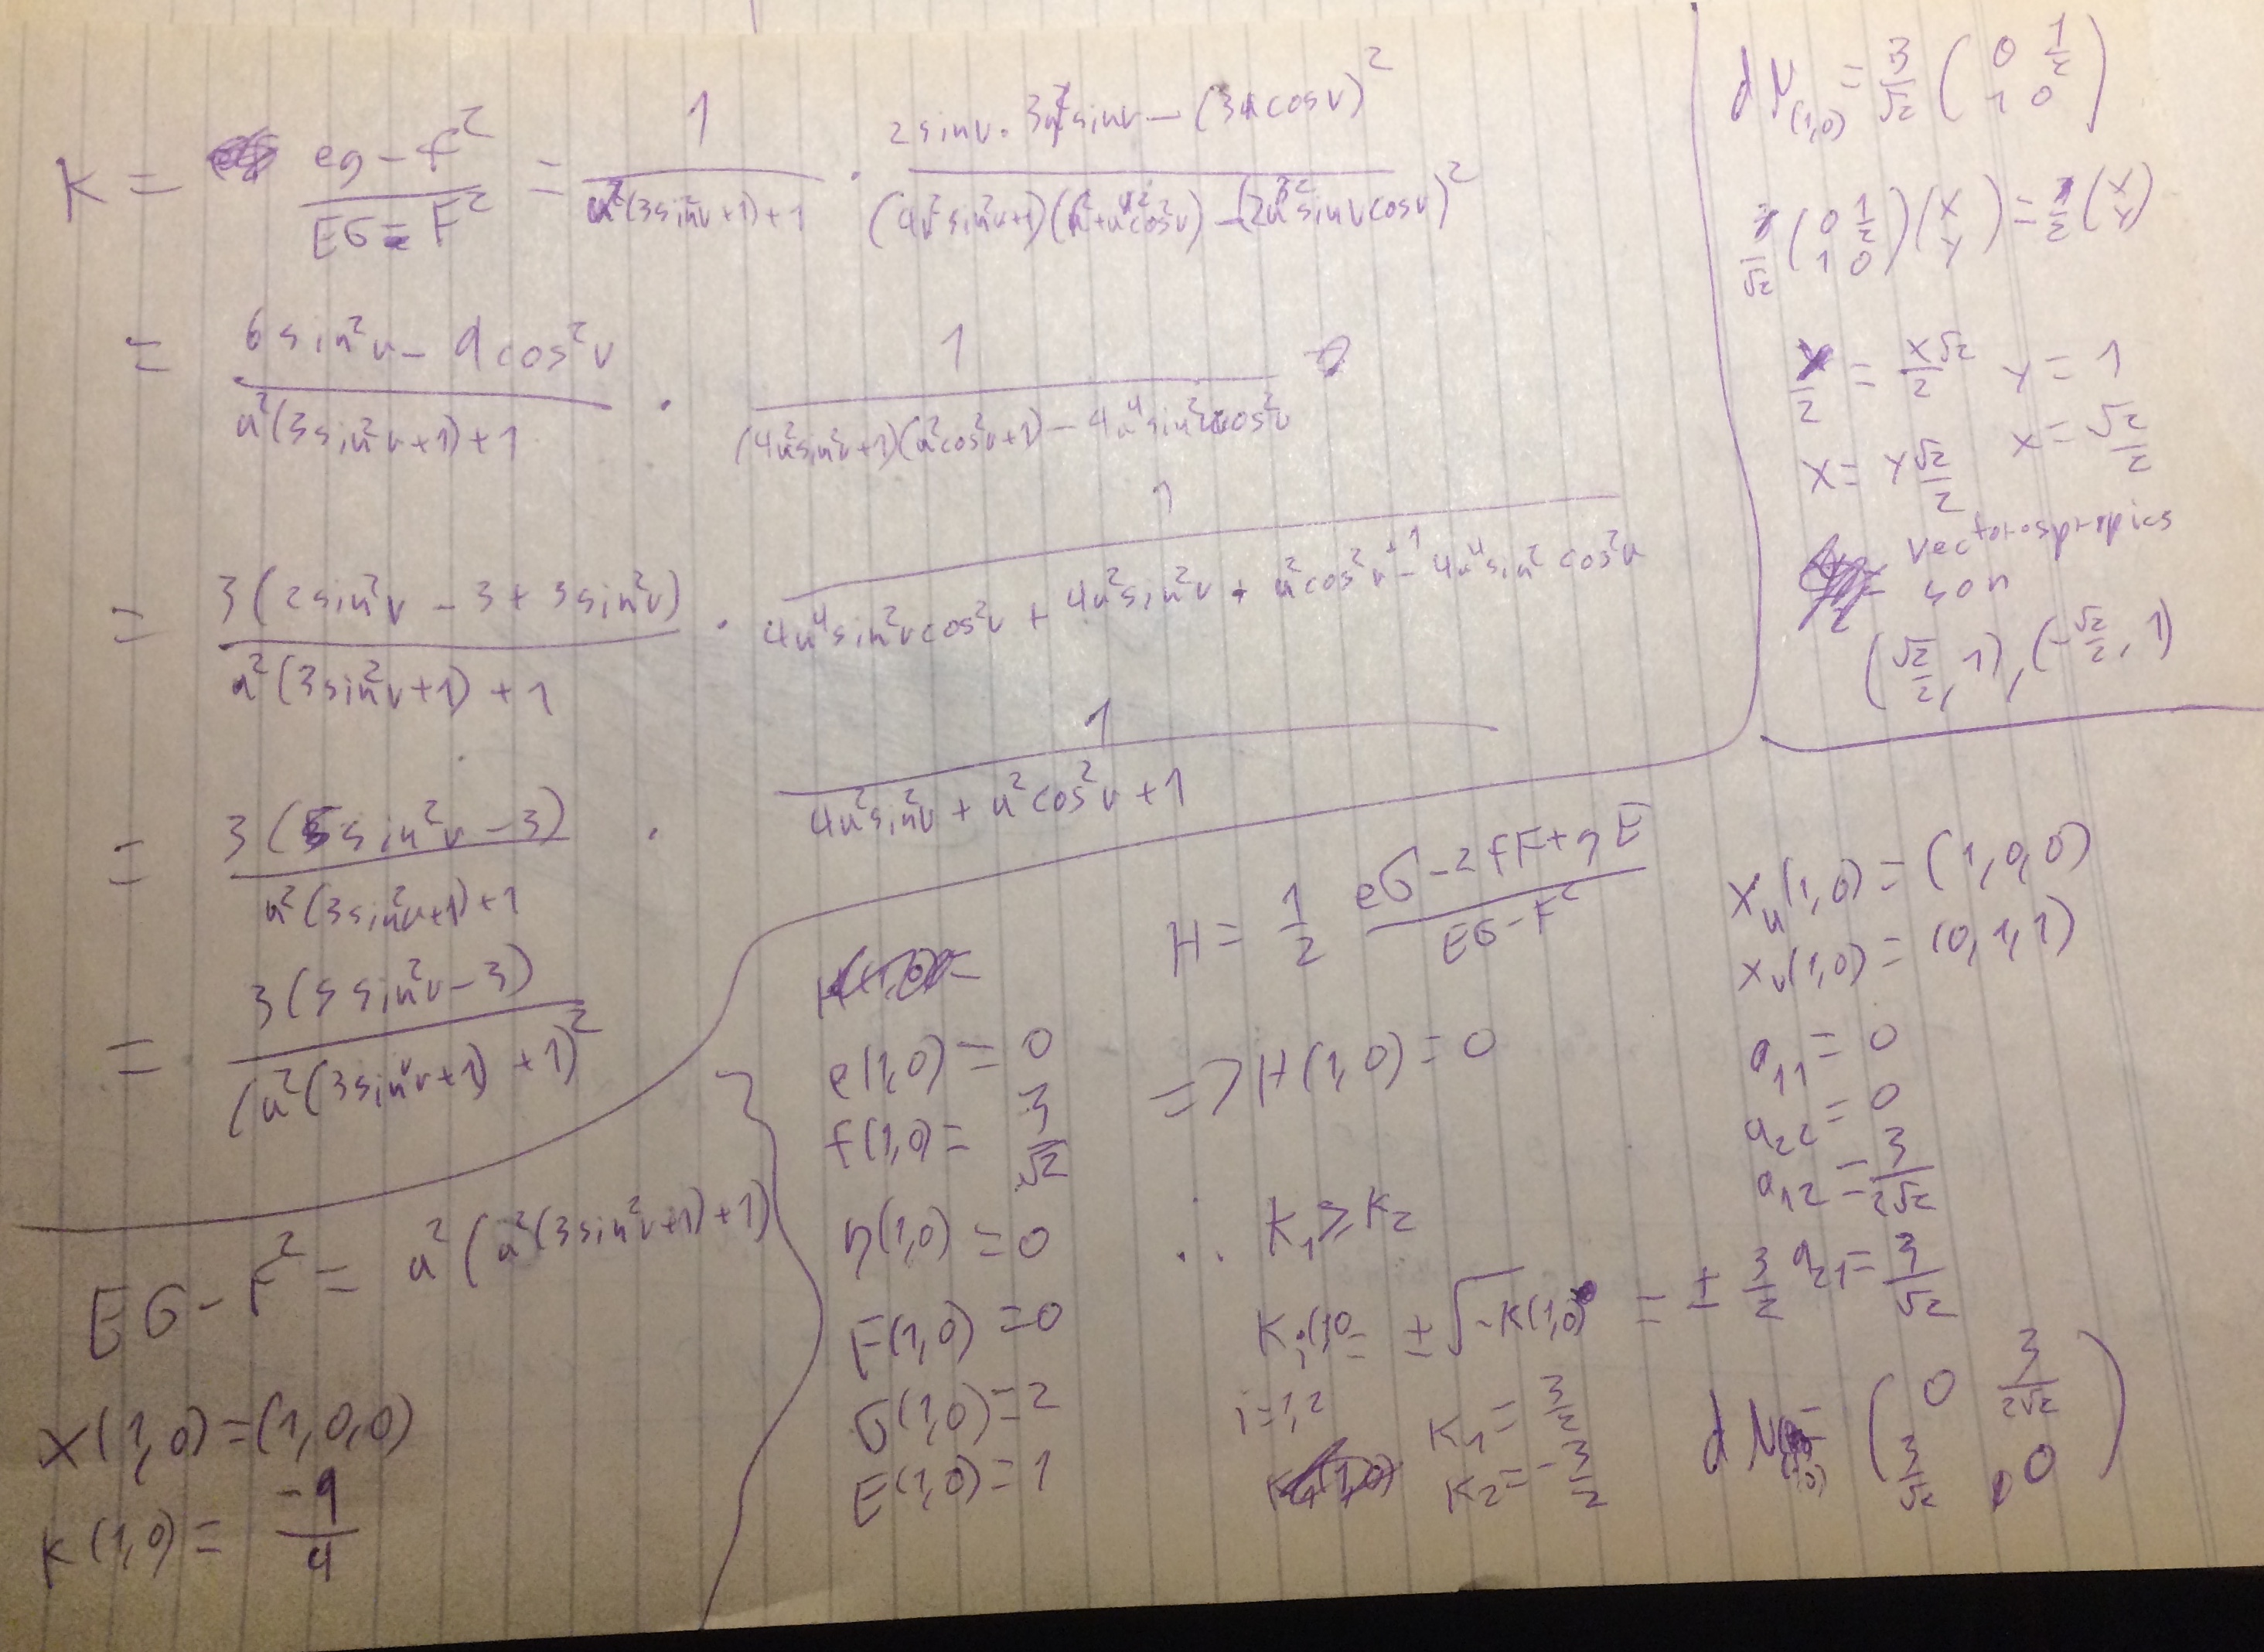
\includegraphics{img/IMG_5985.JPG}
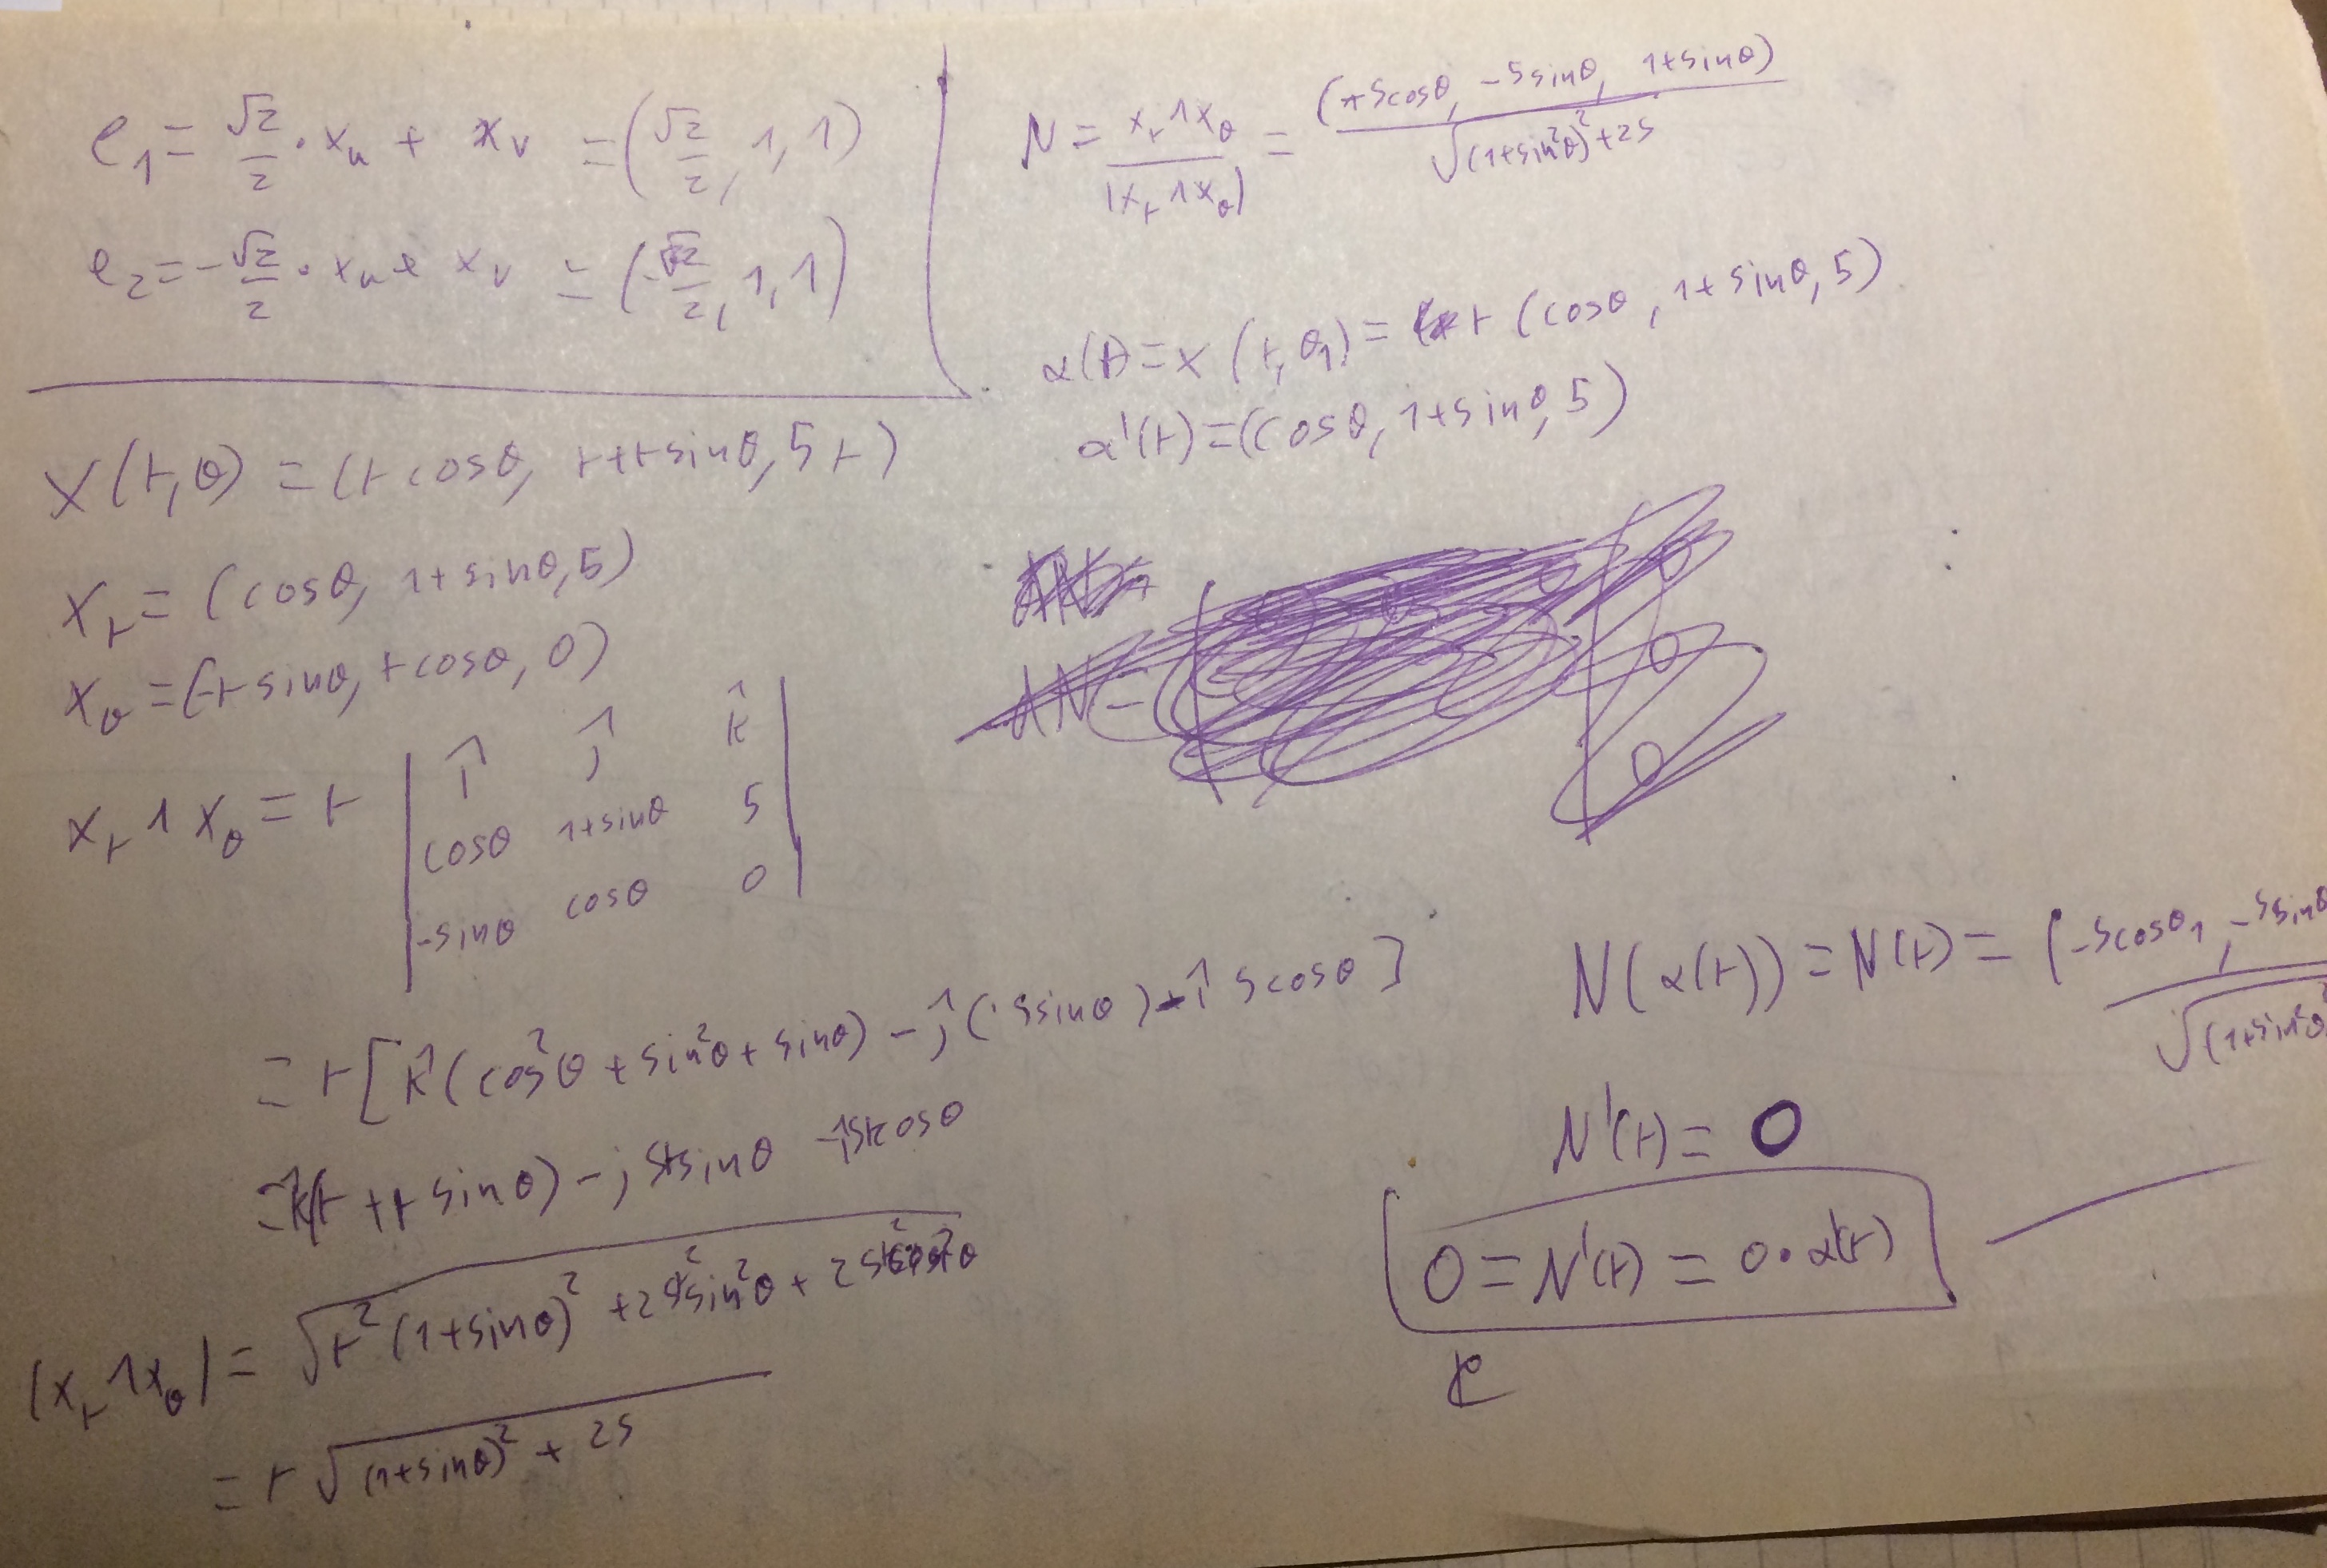
\includegraphics{img/IMG_5986.JPG}
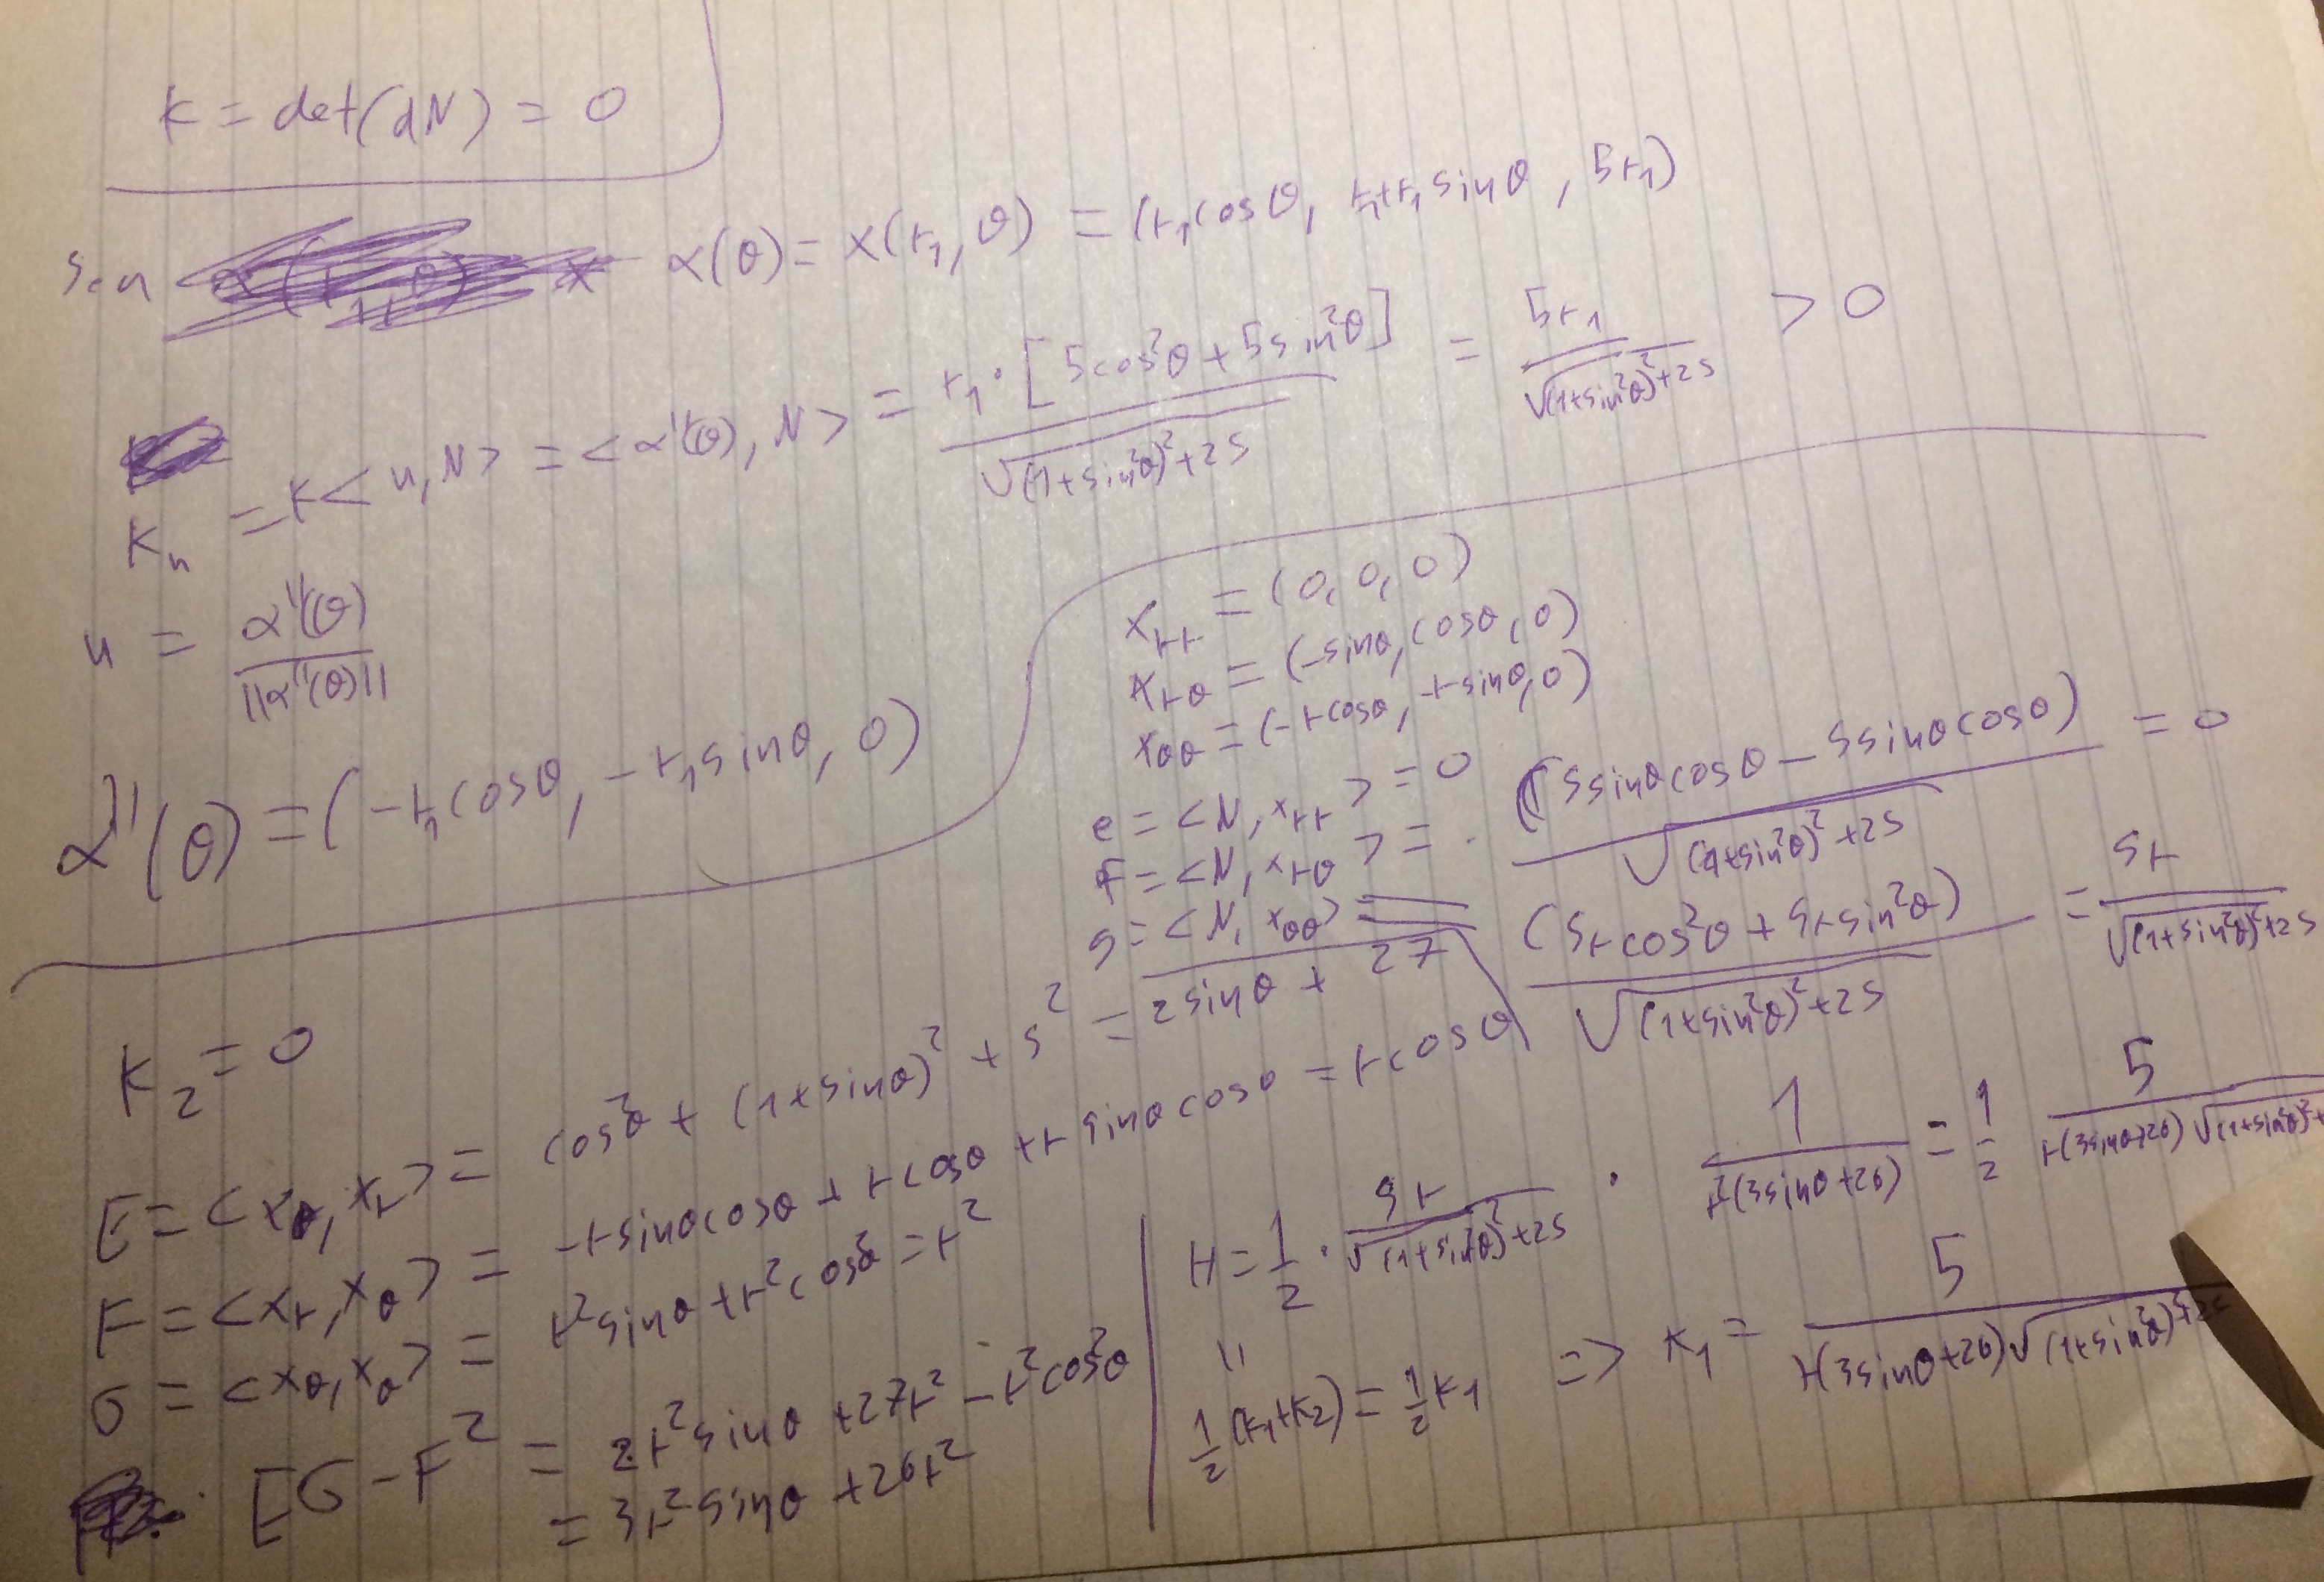
\includegraphics{img/IMG_5987.JPG}
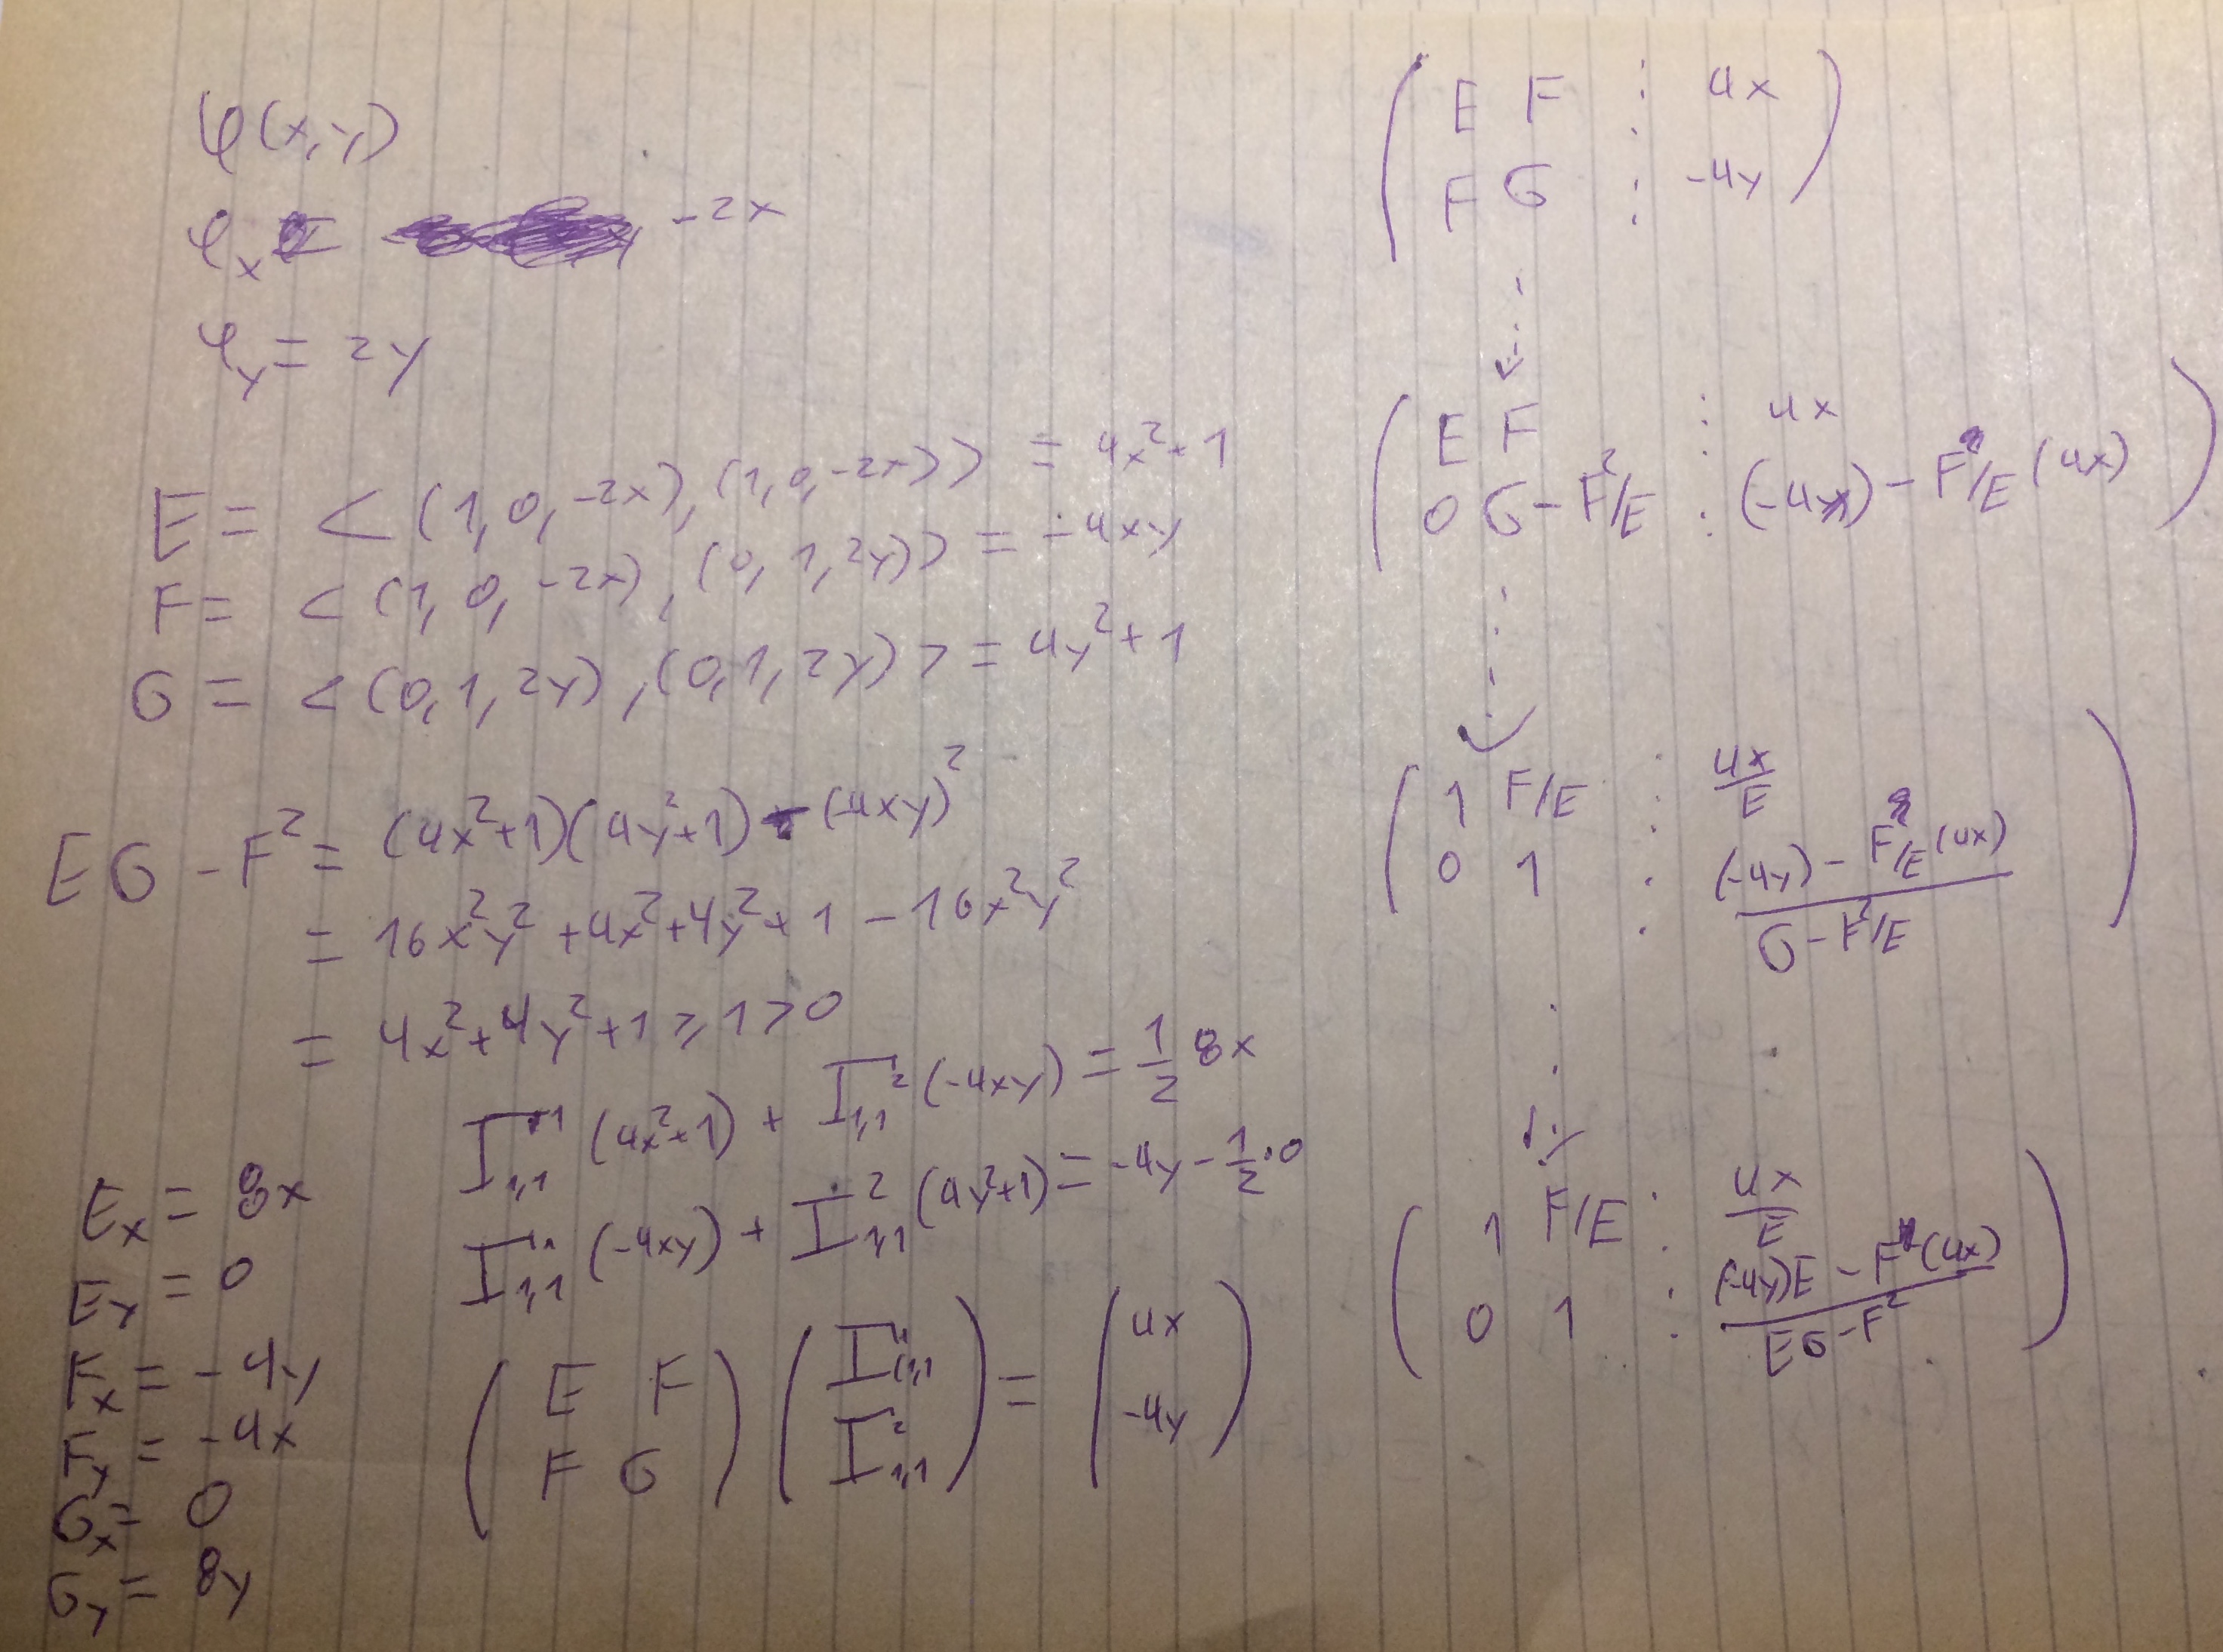
\includegraphics{img/IMG_5988.JPG}
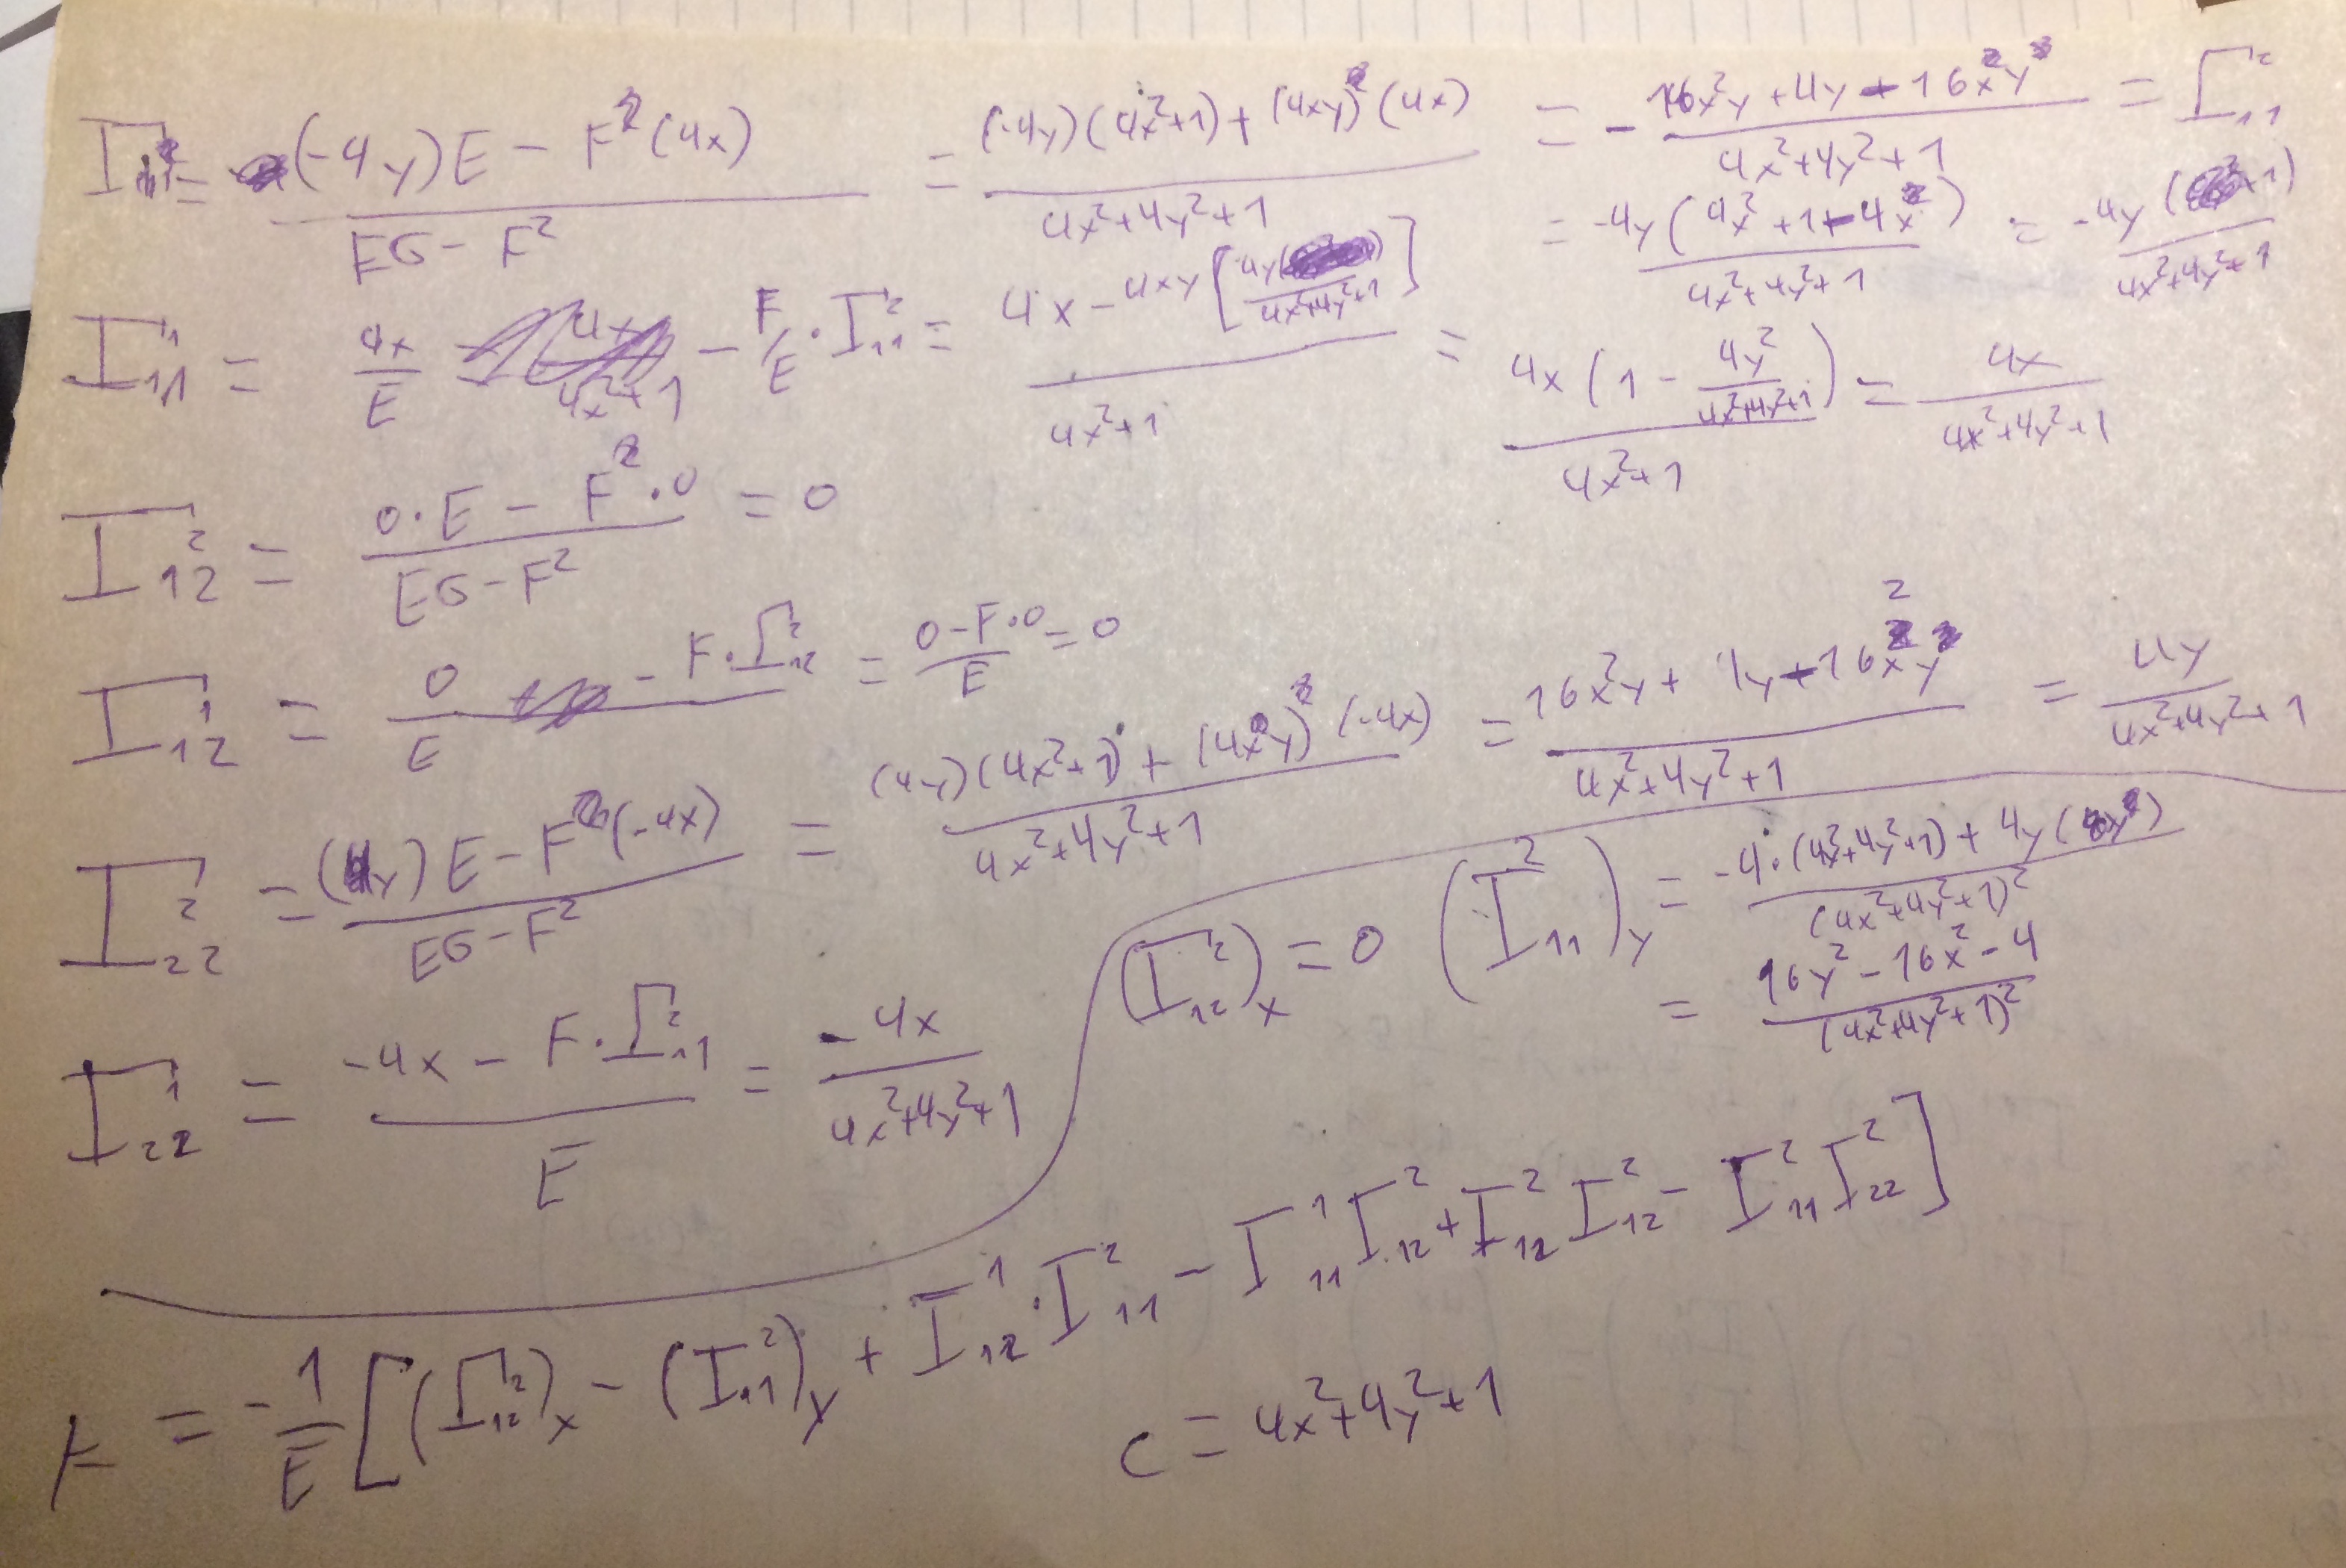
\includegraphics{img/IMG_5989.JPG}
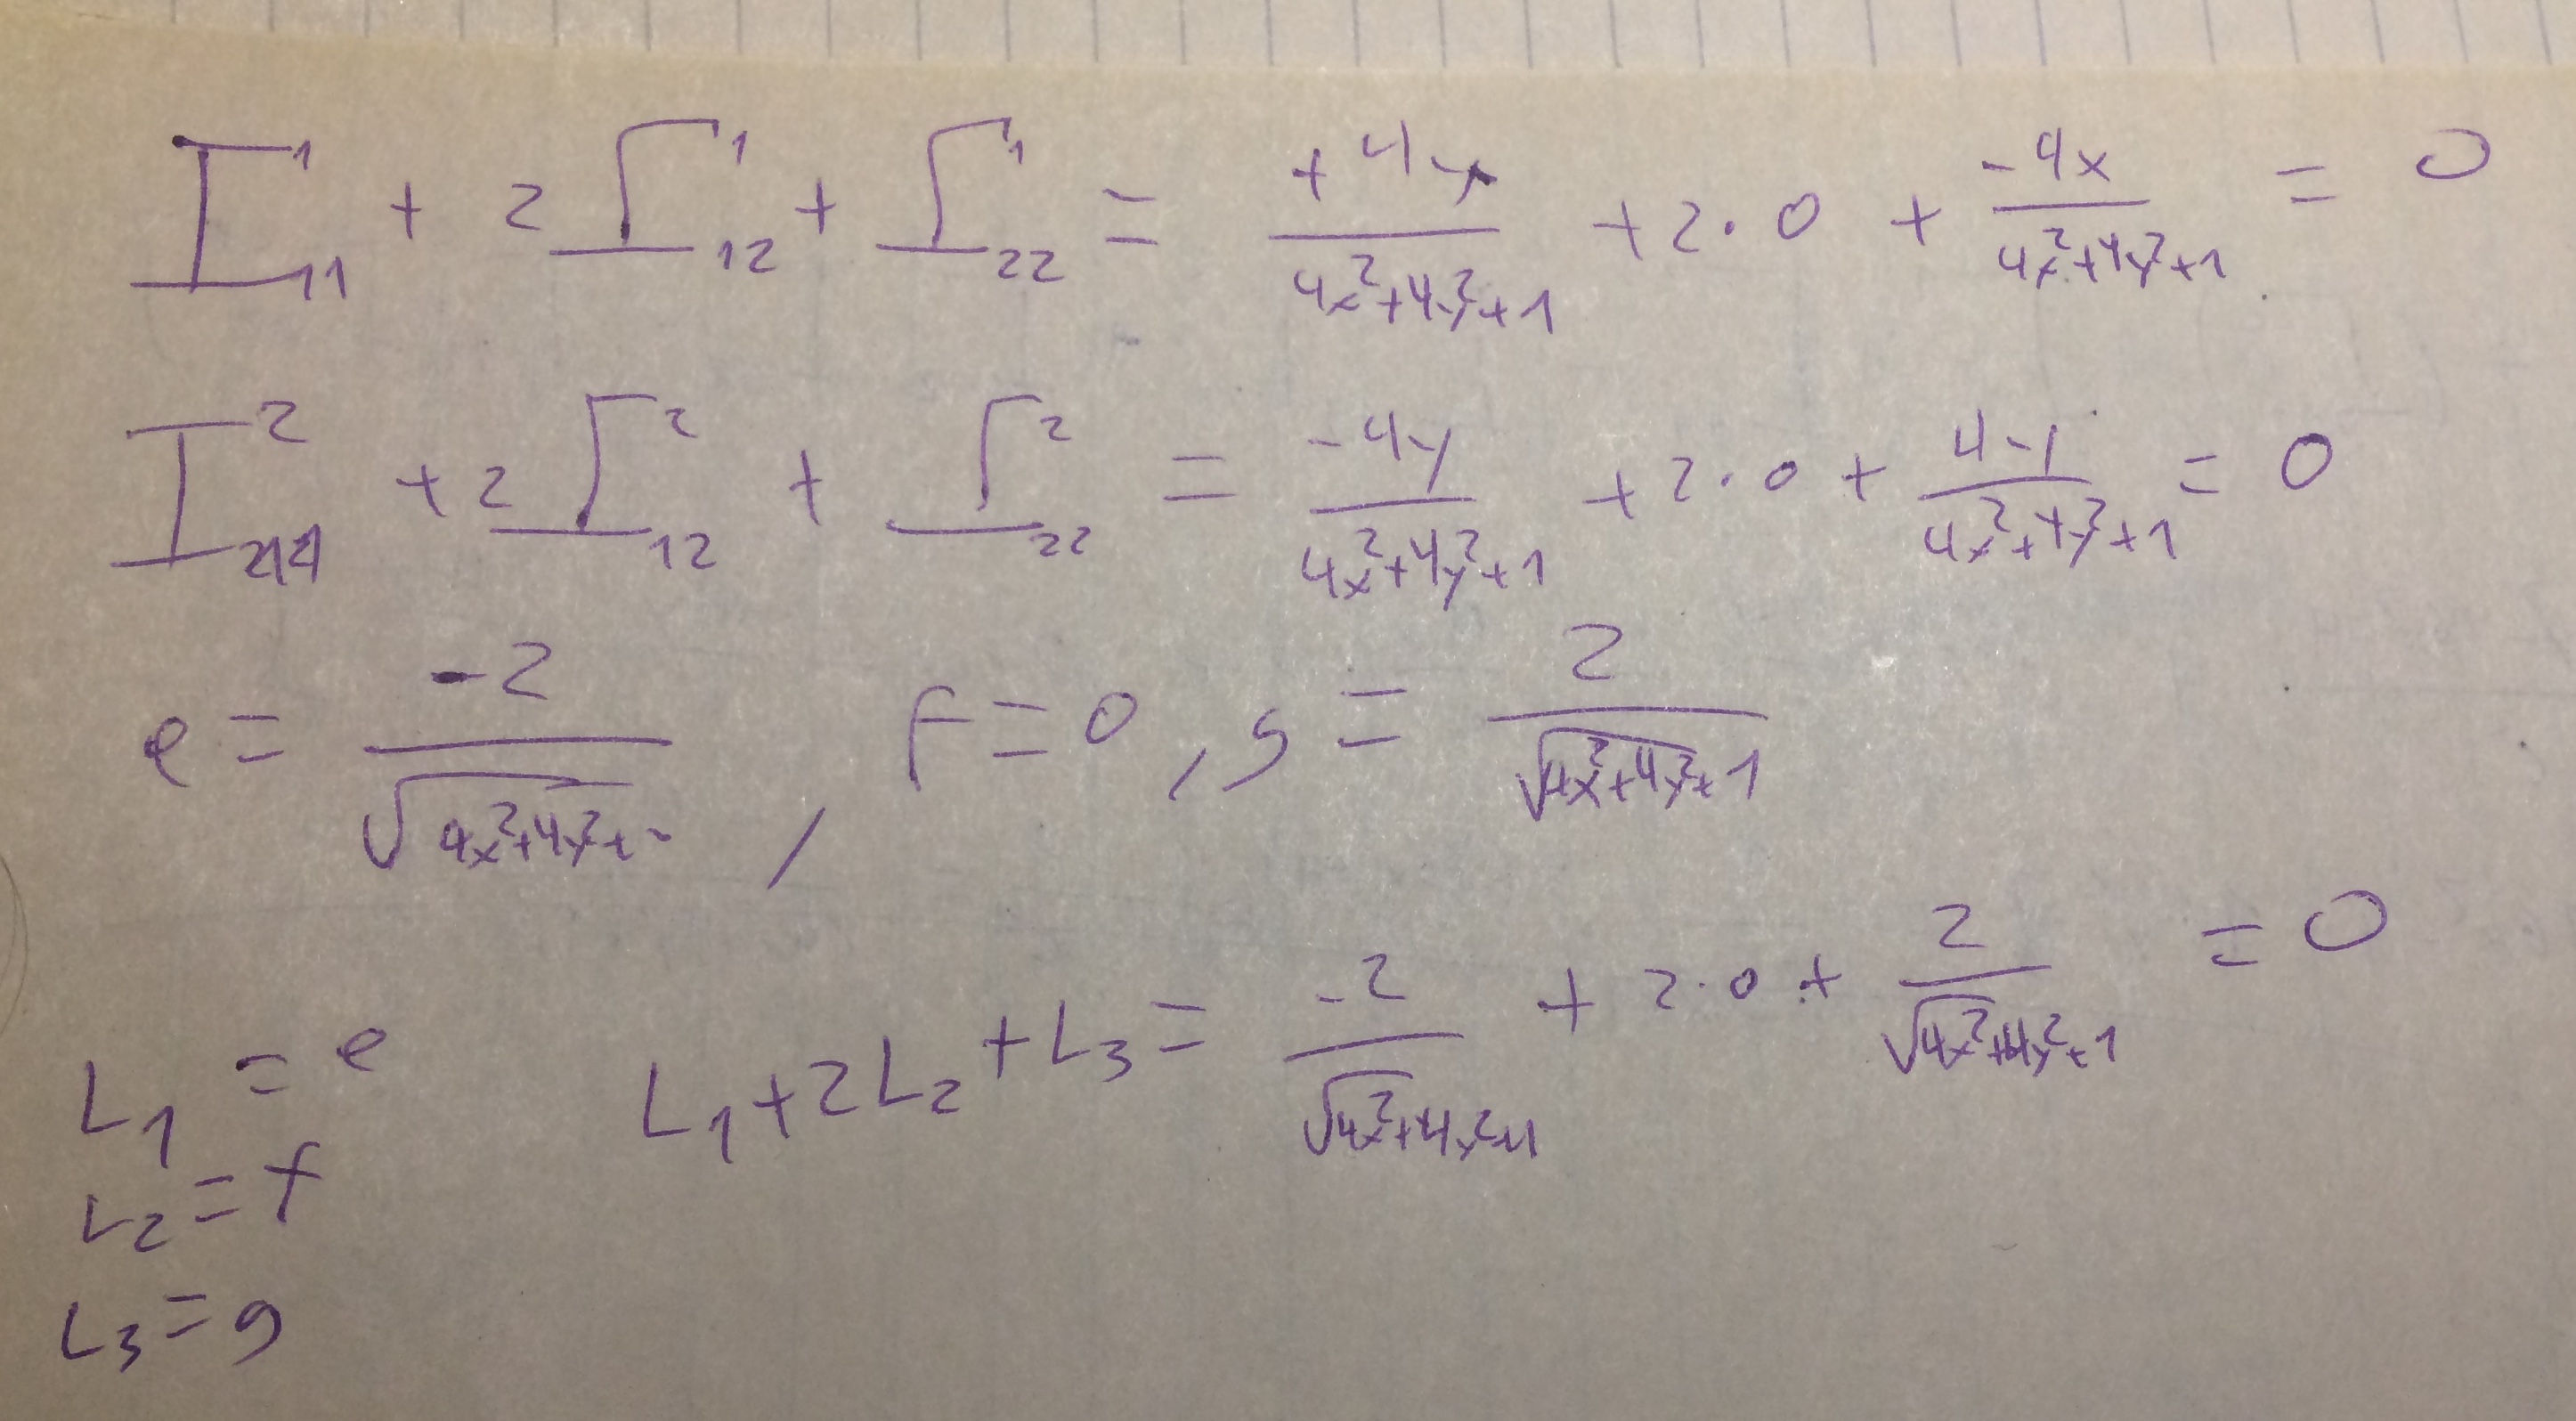
\includegraphics{img/IMG_5990.JPG}
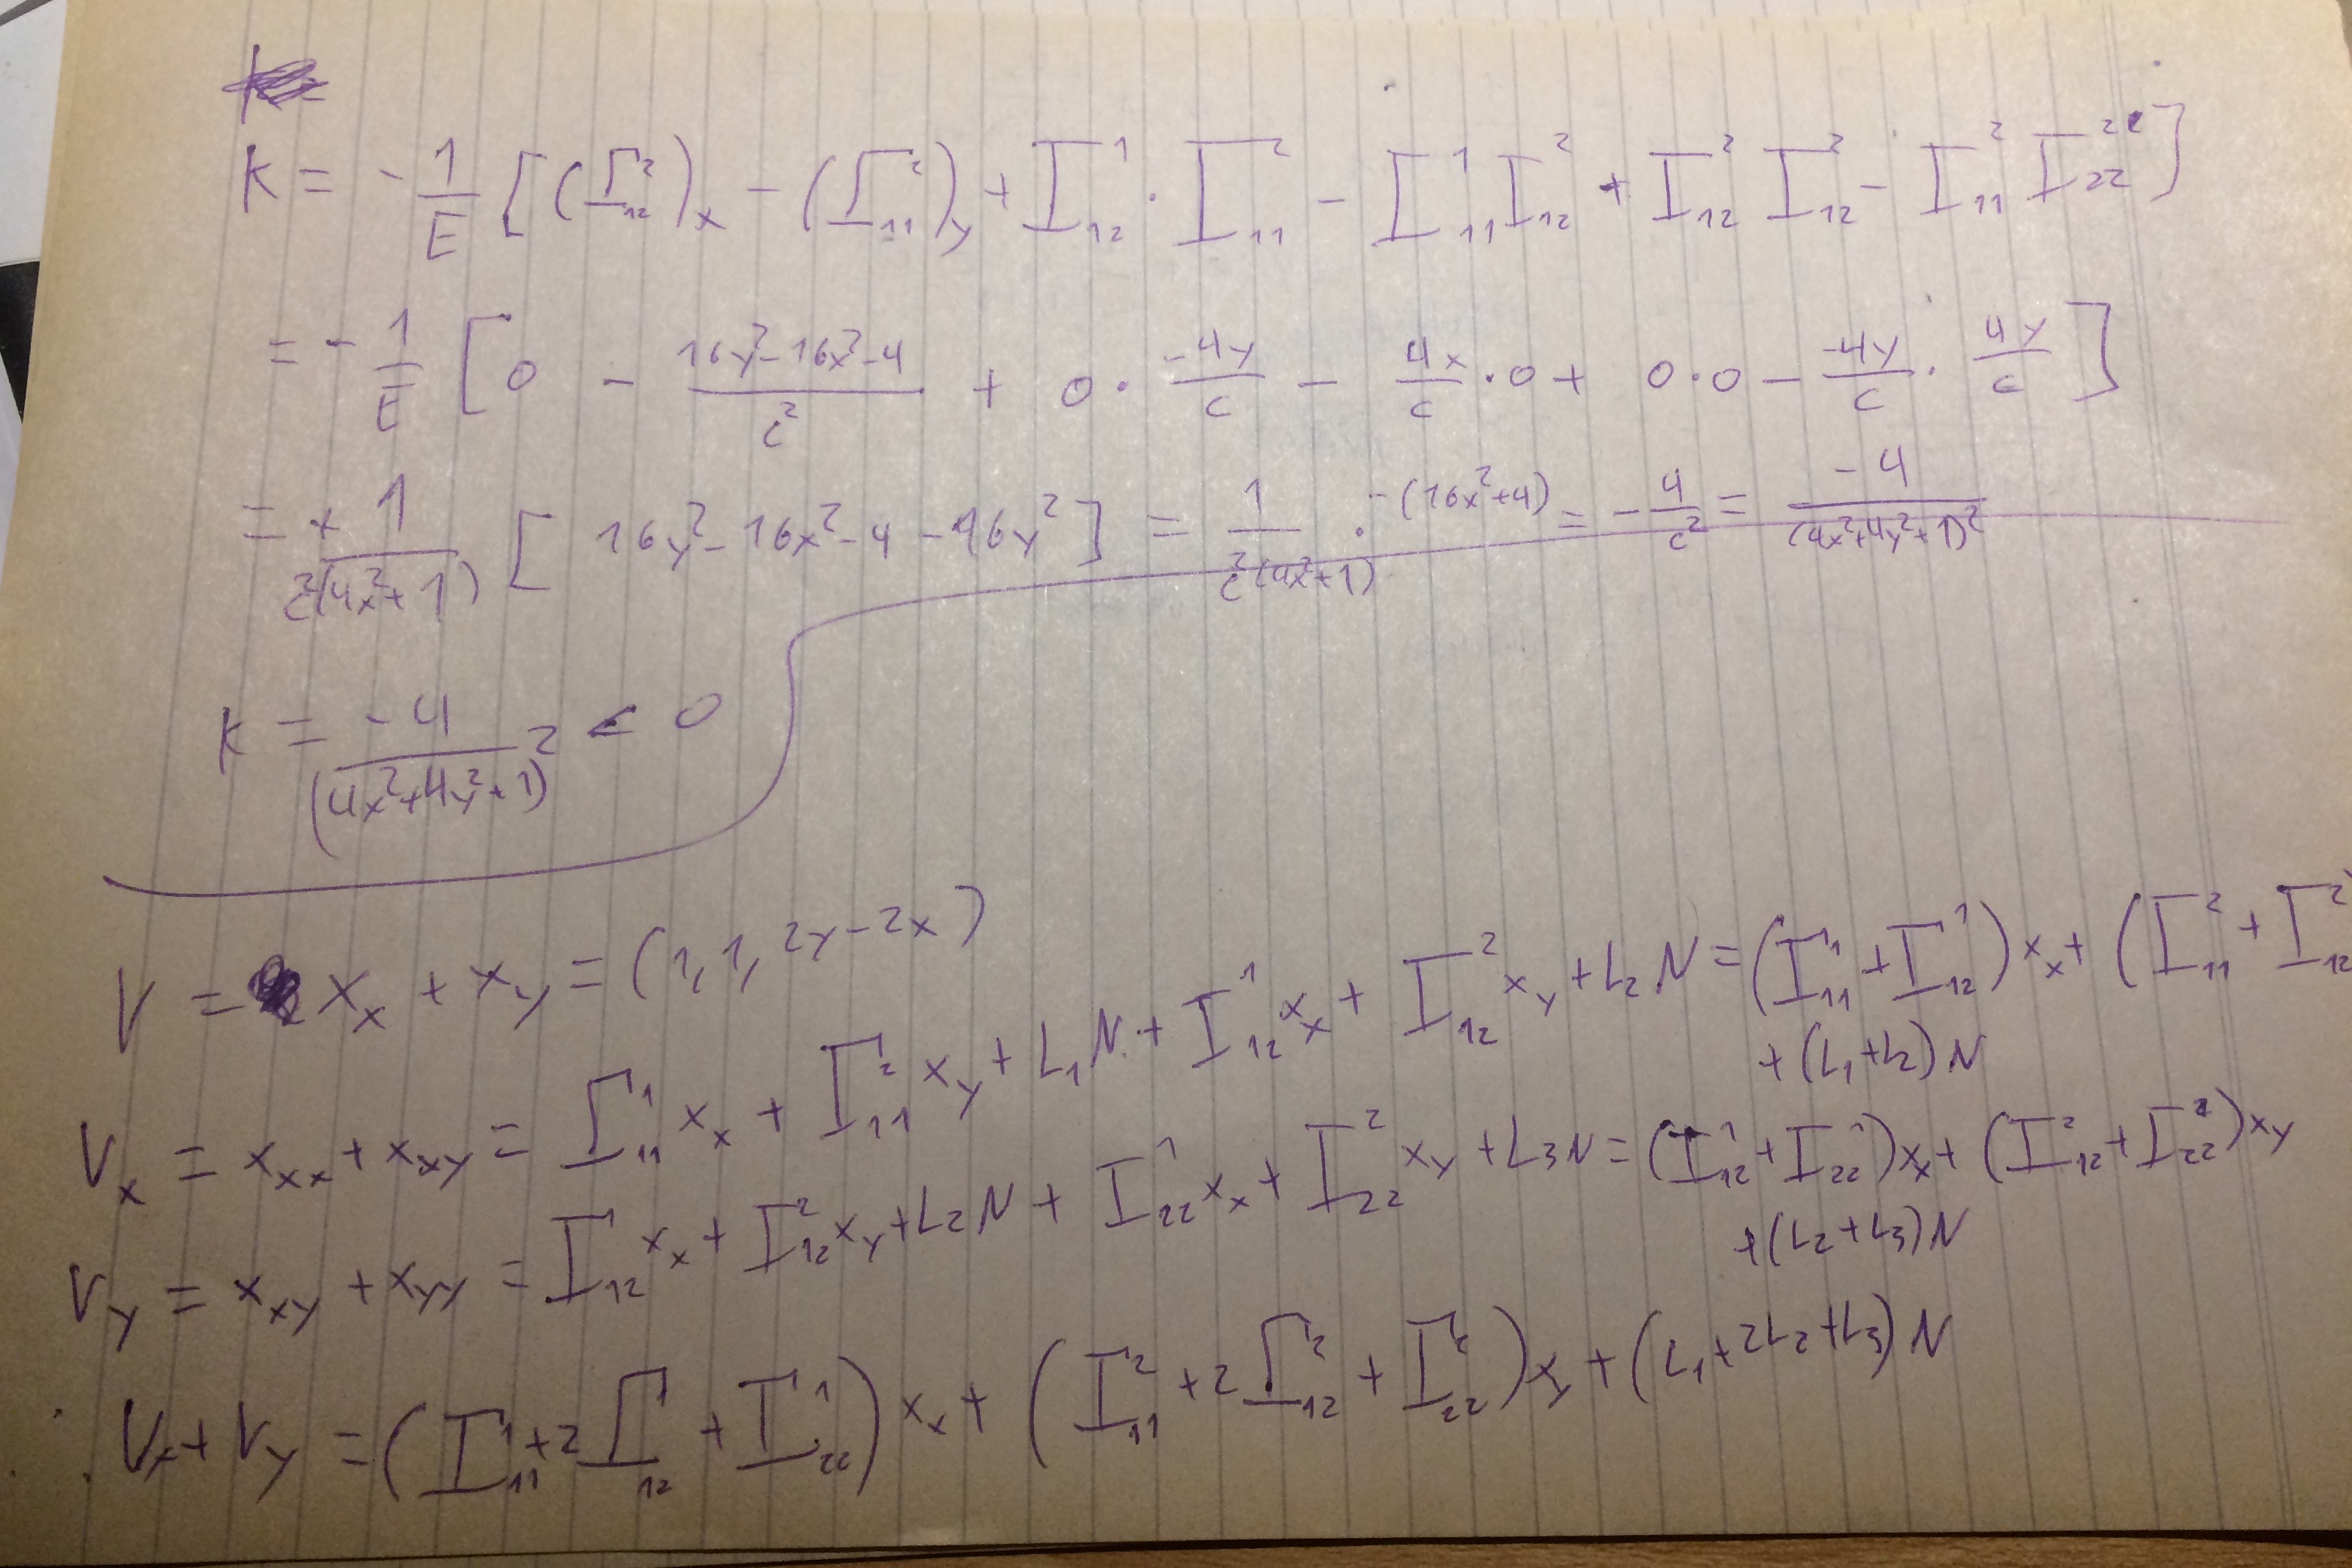
\includegraphics{img/IMG_5991.JPG}

% \end{center}

\end{document}